% Options for packages loaded elsewhere
\PassOptionsToPackage{unicode}{hyperref}
\PassOptionsToPackage{hyphens}{url}
%
\documentclass[
]{article}
\usepackage{amsmath,amssymb}
\usepackage{iftex}
\ifPDFTeX
  \usepackage[T1]{fontenc}
  \usepackage[utf8]{inputenc}
  \usepackage{textcomp} % provide euro and other symbols
\else % if luatex or xetex
  \usepackage{unicode-math} % this also loads fontspec
  \defaultfontfeatures{Scale=MatchLowercase}
  \defaultfontfeatures[\rmfamily]{Ligatures=TeX,Scale=1}
\fi
\usepackage{lmodern}
\ifPDFTeX\else
  % xetex/luatex font selection
\fi
% Use upquote if available, for straight quotes in verbatim environments
\IfFileExists{upquote.sty}{\usepackage{upquote}}{}
\IfFileExists{microtype.sty}{% use microtype if available
  \usepackage[]{microtype}
  \UseMicrotypeSet[protrusion]{basicmath} % disable protrusion for tt fonts
}{}
\makeatletter
\@ifundefined{KOMAClassName}{% if non-KOMA class
  \IfFileExists{parskip.sty}{%
    \usepackage{parskip}
  }{% else
    \setlength{\parindent}{0pt}
    \setlength{\parskip}{6pt plus 2pt minus 1pt}}
}{% if KOMA class
  \KOMAoptions{parskip=half}}
\makeatother
\usepackage{xcolor}
\usepackage[margin=1in]{geometry}
\usepackage{color}
\usepackage{fancyvrb}
\newcommand{\VerbBar}{|}
\newcommand{\VERB}{\Verb[commandchars=\\\{\}]}
\DefineVerbatimEnvironment{Highlighting}{Verbatim}{commandchars=\\\{\}}
% Add ',fontsize=\small' for more characters per line
\usepackage{framed}
\definecolor{shadecolor}{RGB}{248,248,248}
\newenvironment{Shaded}{\begin{snugshade}}{\end{snugshade}}
\newcommand{\AlertTok}[1]{\textcolor[rgb]{0.94,0.16,0.16}{#1}}
\newcommand{\AnnotationTok}[1]{\textcolor[rgb]{0.56,0.35,0.01}{\textbf{\textit{#1}}}}
\newcommand{\AttributeTok}[1]{\textcolor[rgb]{0.13,0.29,0.53}{#1}}
\newcommand{\BaseNTok}[1]{\textcolor[rgb]{0.00,0.00,0.81}{#1}}
\newcommand{\BuiltInTok}[1]{#1}
\newcommand{\CharTok}[1]{\textcolor[rgb]{0.31,0.60,0.02}{#1}}
\newcommand{\CommentTok}[1]{\textcolor[rgb]{0.56,0.35,0.01}{\textit{#1}}}
\newcommand{\CommentVarTok}[1]{\textcolor[rgb]{0.56,0.35,0.01}{\textbf{\textit{#1}}}}
\newcommand{\ConstantTok}[1]{\textcolor[rgb]{0.56,0.35,0.01}{#1}}
\newcommand{\ControlFlowTok}[1]{\textcolor[rgb]{0.13,0.29,0.53}{\textbf{#1}}}
\newcommand{\DataTypeTok}[1]{\textcolor[rgb]{0.13,0.29,0.53}{#1}}
\newcommand{\DecValTok}[1]{\textcolor[rgb]{0.00,0.00,0.81}{#1}}
\newcommand{\DocumentationTok}[1]{\textcolor[rgb]{0.56,0.35,0.01}{\textbf{\textit{#1}}}}
\newcommand{\ErrorTok}[1]{\textcolor[rgb]{0.64,0.00,0.00}{\textbf{#1}}}
\newcommand{\ExtensionTok}[1]{#1}
\newcommand{\FloatTok}[1]{\textcolor[rgb]{0.00,0.00,0.81}{#1}}
\newcommand{\FunctionTok}[1]{\textcolor[rgb]{0.13,0.29,0.53}{\textbf{#1}}}
\newcommand{\ImportTok}[1]{#1}
\newcommand{\InformationTok}[1]{\textcolor[rgb]{0.56,0.35,0.01}{\textbf{\textit{#1}}}}
\newcommand{\KeywordTok}[1]{\textcolor[rgb]{0.13,0.29,0.53}{\textbf{#1}}}
\newcommand{\NormalTok}[1]{#1}
\newcommand{\OperatorTok}[1]{\textcolor[rgb]{0.81,0.36,0.00}{\textbf{#1}}}
\newcommand{\OtherTok}[1]{\textcolor[rgb]{0.56,0.35,0.01}{#1}}
\newcommand{\PreprocessorTok}[1]{\textcolor[rgb]{0.56,0.35,0.01}{\textit{#1}}}
\newcommand{\RegionMarkerTok}[1]{#1}
\newcommand{\SpecialCharTok}[1]{\textcolor[rgb]{0.81,0.36,0.00}{\textbf{#1}}}
\newcommand{\SpecialStringTok}[1]{\textcolor[rgb]{0.31,0.60,0.02}{#1}}
\newcommand{\StringTok}[1]{\textcolor[rgb]{0.31,0.60,0.02}{#1}}
\newcommand{\VariableTok}[1]{\textcolor[rgb]{0.00,0.00,0.00}{#1}}
\newcommand{\VerbatimStringTok}[1]{\textcolor[rgb]{0.31,0.60,0.02}{#1}}
\newcommand{\WarningTok}[1]{\textcolor[rgb]{0.56,0.35,0.01}{\textbf{\textit{#1}}}}
\usepackage{graphicx}
\makeatletter
\newsavebox\pandoc@box
\newcommand*\pandocbounded[1]{% scales image to fit in text height/width
  \sbox\pandoc@box{#1}%
  \Gscale@div\@tempa{\textheight}{\dimexpr\ht\pandoc@box+\dp\pandoc@box\relax}%
  \Gscale@div\@tempb{\linewidth}{\wd\pandoc@box}%
  \ifdim\@tempb\p@<\@tempa\p@\let\@tempa\@tempb\fi% select the smaller of both
  \ifdim\@tempa\p@<\p@\scalebox{\@tempa}{\usebox\pandoc@box}%
  \else\usebox{\pandoc@box}%
  \fi%
}
% Set default figure placement to htbp
\def\fps@figure{htbp}
\makeatother
\setlength{\emergencystretch}{3em} % prevent overfull lines
\providecommand{\tightlist}{%
  \setlength{\itemsep}{0pt}\setlength{\parskip}{0pt}}
\setcounter{secnumdepth}{5}
\usepackage{booktabs}
\usepackage{longtable}
\usepackage{array}
\usepackage{multirow}
\usepackage{wrapfig}
\usepackage{float}
\usepackage{colortbl}
\usepackage{pdflscape}
\usepackage{tabu}
\usepackage{threeparttable}
\usepackage{threeparttablex}
\usepackage[normalem]{ulem}
\usepackage{makecell}
\usepackage{xcolor}
\usepackage{bookmark}
\IfFileExists{xurl.sty}{\usepackage{xurl}}{} % add URL line breaks if available
\urlstyle{same}
\hypersetup{
  pdftitle={Einfluss der Wettbewerbsstruktur auf Gehaltsniveaus im Data Science-Bereich:},
  hidelinks,
  pdfcreator={LaTeX via pandoc}}

\title{Einfluss der Wettbewerbsstruktur auf Gehaltsniveaus im Data
Science-Bereich:}
\usepackage{etoolbox}
\makeatletter
\providecommand{\subtitle}[1]{% add subtitle to \maketitle
  \apptocmd{\@title}{\par {\large #1 \par}}{}{}
}
\makeatother
\subtitle{Eine Social Network Analyse}
\author{}
\date{\vspace{-2.5em}}

\begin{document}
\maketitle

{
\setcounter{tocdepth}{3}
\tableofcontents
}
\newpage

\section{Einleitung}\label{einleitung}

\subsection{Requirements}\label{requirements}

Zunächst müssen die benötigten Bibliotheken installiert werden:

\begin{itemize}
\tightlist
\item
  \$ install.packages(``tidyverse'')
\item
  \$ install.packages(``igraph'')
\item
  \$ install.packages(``visNetwork'')
\item
  \$ install.packages(``dplyr'')
\item
  \$ install.packages(``tidyr'')
\item
  \$ install.packages(``kableExtra'')
\item
  \$ install.packages(``webshot'')
\item
  \$ install.packages(``knitr'')
\item
  \$ install.packages(``ggplot2'')
\item
  \$ install.packages(``RColorBrewer'')
\end{itemize}

Und anschließend geladen werden:

\begin{Shaded}
\begin{Highlighting}[]
\FunctionTok{library}\NormalTok{(tidyverse)}
\FunctionTok{library}\NormalTok{(igraph)}
\FunctionTok{library}\NormalTok{(visNetwork)}
\FunctionTok{library}\NormalTok{(dplyr)}
\FunctionTok{library}\NormalTok{(tidyr)}
\FunctionTok{library}\NormalTok{(knitr)}
\FunctionTok{library}\NormalTok{(kableExtra)}
\FunctionTok{library}\NormalTok{(webshot)}
\FunctionTok{library}\NormalTok{(ggplot2)}
\FunctionTok{library}\NormalTok{(RColorBrewer)}
\end{Highlighting}
\end{Shaded}

\subsection{Motivation und
Zielsetzung}\label{motivation-und-zielsetzung}

In ihrem Artikel ``Data Scientist: The Sexiest Job of the 21st Century''
betonen Davenport und Patil, dass Data Scientists durch ihre Fähigkeiten
in Informatik, Statistik und ihr Fachwissen allgemein einen erheblichen
Mehrwert für Unternehmen schaffen.\footnote{Davenport, Patil 2012} Die
Fähigkeit, aus komplexen, unstrukturierten Daten wertvolle Erkenntnisse
zu gewinnen, macht Data Scientisten in vielen Branchen zu einer
unverzichtbaren Ressource.\footnote{Davenport, Patil 2012} Die Nutzung
ihrer Kompetenzen verschafft Unternehmen einen Wettbewerbsvorteil, da
sie datengetriebene Entscheidungen, Produktinnovationen und
Effizienzsteigerungen ermöglicht.\footnote{Davenport, Patil 2012}

Darüber ob Data Scientists immer noch the ``Sexiest Job'' des 21.
Jahrhunderts sind, lässt sich streiten. Fakt ist jedoch, dass die
Nachfrage nach Data Scientists in den letzten Jahren stark gestiegen ist
und vorraussichtlich immer weiter steigen wird. Dieser Trend ist auch in
den Google-Suchanfragen zu den Begriffen erkenntlich:\footnote{Google
  Trends, abgerufen am 30.10.2024}

\begin{Shaded}
\begin{Highlighting}[]
\FunctionTok{ggplot}\NormalTok{(data, }\FunctionTok{aes}\NormalTok{(}\AttributeTok{x =}\NormalTok{ Monat)) }\SpecialCharTok{+}
  \FunctionTok{geom\_line}\NormalTok{(}\FunctionTok{aes}\NormalTok{(}\AttributeTok{y =} \StringTok{\textasciigrave{}}\AttributeTok{data science}\StringTok{\textasciigrave{}}\NormalTok{, }\AttributeTok{color =} \StringTok{"data science"}\NormalTok{)) }\SpecialCharTok{+}
  \FunctionTok{geom\_line}\NormalTok{(}\FunctionTok{aes}\NormalTok{(}\AttributeTok{y =} \StringTok{\textasciigrave{}}\AttributeTok{data scientist}\StringTok{\textasciigrave{}}\NormalTok{, }\AttributeTok{color =} \StringTok{"data scientist"}\NormalTok{)) }\SpecialCharTok{+}
  \FunctionTok{labs}\NormalTok{(}\AttributeTok{title =} \StringTok{"Google Suchtrend für \textquotesingle{}data science\textquotesingle{} und \textquotesingle{}data scientist\textquotesingle{}"}\NormalTok{,}
       \AttributeTok{x =} \StringTok{"Datum"}\NormalTok{,}
       \AttributeTok{y =} \StringTok{"Interesse"}\NormalTok{,}
       \AttributeTok{color =} \StringTok{"Suchbegriff"}\NormalTok{) }\SpecialCharTok{+}
  \FunctionTok{theme\_minimal}\NormalTok{()}
\end{Highlighting}
\end{Shaded}

\pandocbounded{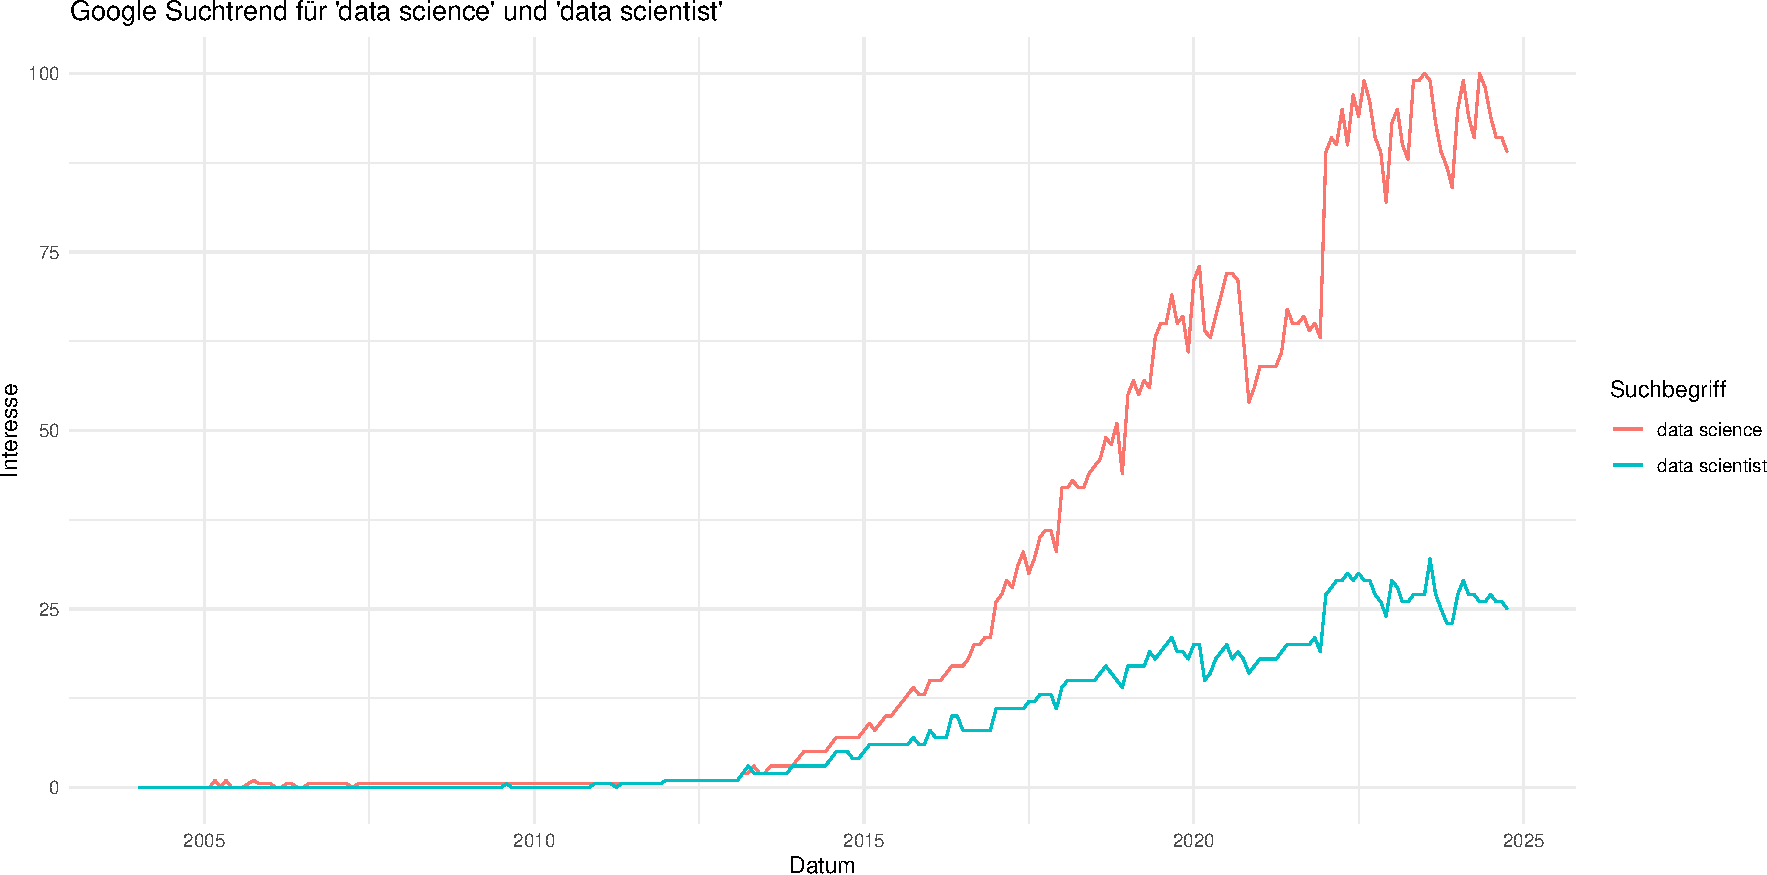
\includegraphics[keepaspectratio]{DataScience_files/figure-latex/unnamed-chunk-2-1.pdf}}

Das wachsende Interesse an Data Science stellt eine große Chance für
Arbeitnehmer dar. Ziel dieser Arbeit ist es einen Überblick über den
Data-Science-Jobmarkt zu geben, um Arbeitnehmern bei der Jobsuche zu
helfen und andererseits einen Überblick über die Gehälter und die Rolle
von Geographie und Wettbewerb bei Jobangeboten und Gehältern zu geben.

\subsection{Forschungsfrage}\label{forschungsfrage}

Im Rahmen der vorliegenden Arbeit wird die folgende Forschungsfrage
bearbeitet:

Inwiefern beeinflusst die geografische Nähe von Unternehmen das
Gehaltsniveau und die Verfügbarkeit von Data-Science-Jobs? Lässt sich
eine signifikante Variation der Einkommen innerhalb regionaler Cluster
feststellen, und wie kann diese durch Netzwerkzentralität erklärt
werden?

Zur Beantwortung dieser Forschungsfrage soll zudem analysiert werden,
inwiefern das Wettbewerbsumfeld zwischen Unternehmen die Gehaltsstruktur
im Bereich Data Science beeinflusst und welche Rolle zentrale
Unternehmen bei der Bestimmung des Gehaltsniveaus spielen.

\subsection{Datengrundlage}\label{datengrundlage}

Nachdem die Daten in Python extern als Vorbereitung aufbereitet wurden,
kann nun die Datengrundlage für diese Arbeit in R eingelesen werden.
Dabei wurde sich an
\url{https://www.kaggle.com/code/fahadrehman07/data-science-job-salary-prediction-glassdoor}
orientiert.

\subsubsection{CSV einlesen}\label{csv-einlesen}

\begin{Shaded}
\begin{Highlighting}[]
\NormalTok{data }\OtherTok{\textless{}{-}} \FunctionTok{read\_csv}\NormalTok{(}\StringTok{"data/Glassdoor\_DataScience\_Salary.csv"}\NormalTok{)}
\end{Highlighting}
\end{Shaded}

\begin{verbatim}
## Rows: 742 Columns: 28
## -- Column specification --------------------------------------------------------
## Delimiter: ","
## chr (14): Job Title, Job Description, Company Name, Location, Headquarters, ...
## dbl (14): Salary Estimate, Rating, Founded, Min_Salary, Max_Salary, Same Sta...
## 
## i Use `spec()` to retrieve the full column specification for this data.
## i Specify the column types or set `show_col_types = FALSE` to quiet this message.
\end{verbatim}

Die vorliegende Arbeit basiert auf einem Datensatz von Kaggle, der
Informationen über Data Science Jobs in verschiedenen Unternehmen für
den US-amerikanischen Markt enthält. Der Datensatz umfasst 742 Zeilen
und 28 Spalten, was auf eine Anzahl von 742 verschiedenen Jobangeboten
hindeutet. Diese Anzahl ist kann für die Zwecke dieser Arbeit als
ausreichend zu betrachten, auch wenn eine höhere Zahl an Beobachtungen
möglicherweise zu präziseren Schlussfolgerungen geführt hätte.

Der Datensatz beruht auf Daten, die von Glassdoor extrahiert wurden,
eine für Stellenanzeigen und Unternehmensbewertung bekannte Website, und
bietet detaillierte Informationen über Data-Science-Jobs sowie deren
Gehälter. Der Datensatz beinhaltet wesentliche Informationen, darunter
Jobtitel, geschätzte Gehälter, Stellenbeschreibungen,
Unternehmensbewertungen sowie relevante Unternehmensdaten wie Standort,
Größe und Branche. Eine detaillierte Beschreibung dieser Daten erfolgt
im späteren Verlauf. Der Datensatz eignet sich in besonderem Maße für
den Zweck dieser Arbeit, aber auch für Analysen des Arbeitsmarktes,
beispielsweise zur Untersuchung von Gehaltstrends oder zur
Identifizierung der am besten bewerteten Unternehmen.

Der Datensatz umfasst konkret die folgenden Spalten:

\subsubsection{Erste Ansicht der Daten}\label{erste-ansicht-der-daten}

\begin{Shaded}
\begin{Highlighting}[]
\FunctionTok{head}\NormalTok{(data, }\DecValTok{5}\NormalTok{)}
\end{Highlighting}
\end{Shaded}

\begin{verbatim}
## # A tibble: 5 x 28
##   `Job Title` `Salary Estimate` `Job Description` Rating `Company Name` Location
##   <chr>                   <dbl> <chr>              <dbl> <chr>          <chr>   
## 1 Data Scien~              72   "Data Scientist\~    3.8 Tecolote Rese~ Albuque~
## 2 Healthcare~              87.5 "What You Will D~    3.4 University of~ Linthic~
## 3 Data Scien~              85   "KnowBe4, Inc. i~    4.8 KnowBe4        Clearwa~
## 4 Data Scien~              76.5 "*Organization a~    3.8 PNNL           Richlan~
## 5 Data Scien~             114.  "Data Scientist\~    2.9 Affinity Solu~ New Yor~
## # i 22 more variables: Headquarters <chr>, Size <chr>, Founded <dbl>,
## #   `Type of ownership` <chr>, Industry <chr>, Sector <chr>, Revenue <chr>,
## #   Competitors <chr>, Min_Salary <dbl>, Max_Salary <dbl>, State <chr>,
## #   `Same State` <dbl>, Age <dbl>, Python_yn <dbl>, `R Studio` <dbl>,
## #   Spark <dbl>, AWS_yn <dbl>, Excel_yn <dbl>, Job_simp <chr>, job_state <chr>,
## #   desc_len <dbl>, Num_comp <dbl>
\end{verbatim}

\begin{Shaded}
\begin{Highlighting}[]
\FunctionTok{spec}\NormalTok{(data)}
\end{Highlighting}
\end{Shaded}

\begin{verbatim}
## cols(
##   `Job Title` = col_character(),
##   `Salary Estimate` = col_double(),
##   `Job Description` = col_character(),
##   Rating = col_double(),
##   `Company Name` = col_character(),
##   Location = col_character(),
##   Headquarters = col_character(),
##   Size = col_character(),
##   Founded = col_double(),
##   `Type of ownership` = col_character(),
##   Industry = col_character(),
##   Sector = col_character(),
##   Revenue = col_character(),
##   Competitors = col_character(),
##   Min_Salary = col_double(),
##   Max_Salary = col_double(),
##   State = col_character(),
##   `Same State` = col_double(),
##   Age = col_double(),
##   Python_yn = col_double(),
##   `R Studio` = col_double(),
##   Spark = col_double(),
##   AWS_yn = col_double(),
##   Excel_yn = col_double(),
##   Job_simp = col_character(),
##   job_state = col_character(),
##   desc_len = col_double(),
##   Num_comp = col_double()
## )
\end{verbatim}

\begin{Shaded}
\begin{Highlighting}[]
\FunctionTok{summary}\NormalTok{(data)}
\end{Highlighting}
\end{Shaded}

\begin{verbatim}
##   Job Title         Salary Estimate Job Description        Rating      
##  Length:742         Min.   : 13.5   Length:742         Min.   :-1.000  
##  Class :character   1st Qu.: 73.5   Class :character   1st Qu.: 3.300  
##  Mode  :character   Median : 97.5   Mode  :character   Median : 3.700  
##                     Mean   :100.6                      Mean   : 3.619  
##                     3rd Qu.:122.5                      3rd Qu.: 4.000  
##                     Max.   :254.0                      Max.   : 5.000  
##  Company Name         Location         Headquarters           Size          
##  Length:742         Length:742         Length:742         Length:742        
##  Class :character   Class :character   Class :character   Class :character  
##  Mode  :character   Mode  :character   Mode  :character   Mode  :character  
##                                                                             
##                                                                             
##                                                                             
##     Founded     Type of ownership    Industry            Sector         
##  Min.   :  -1   Length:742         Length:742         Length:742        
##  1st Qu.:1939   Class :character   Class :character   Class :character  
##  Median :1988   Mode  :character   Mode  :character   Mode  :character  
##  Mean   :1837                                                           
##  3rd Qu.:2007                                                           
##  Max.   :2019                                                           
##    Revenue          Competitors          Min_Salary       Max_Salary   
##  Length:742         Length:742         Min.   : 15.00   Min.   : 16.0  
##  Class :character   Class :character   1st Qu.: 52.00   1st Qu.: 96.0  
##  Mode  :character   Mode  :character   Median : 69.50   Median :124.0  
##                                        Mean   : 74.72   Mean   :127.2  
##                                        3rd Qu.: 91.00   3rd Qu.:155.0  
##                                        Max.   :202.00   Max.   :306.0  
##     State             Same State         Age           Python_yn     
##  Length:742         Min.   :0.000   Min.   : -1.00   Min.   :0.0000  
##  Class :character   1st Qu.:0.000   1st Qu.: 14.00   1st Qu.:0.0000  
##  Mode  :character   Median :1.000   Median : 27.00   Median :1.0000  
##                     Mean   :0.558   Mean   : 49.39   Mean   :0.5283  
##                     3rd Qu.:1.000   3rd Qu.: 62.00   3rd Qu.:1.0000  
##                     Max.   :1.000   Max.   :279.00   Max.   :1.0000  
##     R Studio            Spark            AWS_yn          Excel_yn     
##  Min.   :0.000000   Min.   :0.0000   Min.   :0.0000   Min.   :0.0000  
##  1st Qu.:0.000000   1st Qu.:0.0000   1st Qu.:0.0000   1st Qu.:0.0000  
##  Median :0.000000   Median :0.0000   Median :0.0000   Median :1.0000  
##  Mean   :0.002695   Mean   :0.2251   Mean   :0.2372   Mean   :0.5229  
##  3rd Qu.:0.000000   3rd Qu.:0.0000   3rd Qu.:0.0000   3rd Qu.:1.0000  
##  Max.   :1.000000   Max.   :1.0000   Max.   :1.0000   Max.   :1.0000  
##    Job_simp          job_state            desc_len        Num_comp    
##  Length:742         Length:742         Min.   :  407   Min.   :0.000  
##  Class :character   Class :character   1st Qu.: 2801   1st Qu.:0.000  
##  Mode  :character   Mode  :character   Median : 3731   Median :0.000  
##                                        Mean   : 3870   Mean   :1.054  
##                                        3rd Qu.: 4740   3rd Qu.:3.000  
##                                        Max.   :10051   Max.   :4.000
\end{verbatim}

Im Folgenden wird eine Übersicht der wesentlichen Spalten präsentiert:

\begin{itemize}
\tightlist
\item
  \texttt{Job\ Title}: Die Berufsbezeichnung, sie gibt Aufschluss über
  die Tätigkeit.
\item
  \texttt{Salary\ Estimate}: Die geschätzte Gehalt, in tausend Dollar
  pro Jahr. Es basiert auf dem Durchschnitt von dem minimalen und
  maximalen Gehalt.
\item
  \texttt{Job\ Description}, \texttt{Job\_simp}: Die Beschreibung der
  Stelle, die Aufgaben und Anforderungen enthält. Auch die vereinfachte
  Version der Berufsbezeichnung.
\item
  \texttt{Rating}: Die Bewertung des Unternehmens, sie weist eine
  Spannbreite von 1 bis 5 auf, wobei die Bewertung ``-1'' bei jeder
  Spalte für fehlende Bewertungen steht.
\item
  \texttt{Company\ Name}, \texttt{Location}, \texttt{Headquarters},
  \texttt{Size}, \texttt{Founded}: Unternehmensbezogene Daten wie Name,
  Standort, Sitz, Größe und Gründungsjahr des Unternehmens.
\item
  \texttt{Type\ of\ ownership}, \texttt{Industry}, \texttt{Sector},
  \texttt{Revenue}: Weitere Unternehmensmerkmale, diese umfassen die
  Eigentumsart, die Branche, den Sektor sowie die Einnahmen.
\item
  \texttt{Competitors}: Die Wettbewerber des Unternehmens, die im
  Zusammenhang dieser Arbeit von besonderer Bedeutung sind.
\item
  Skills (\texttt{Python\_yn}, \texttt{R\ Studio}, \texttt{Spark},
  \texttt{AWS\_yn}, \texttt{Excel\_yn}): Spalten, aus denen hervorgeht,
  ob die betreffende Kompetenz in der Stellenbeschreibung verlangt wird
  (0 = nein, 1 = ja).
\item
  \texttt{Min\_salary}, \texttt{Max\_salary}: Minimale und maximale
  Gehaltsschätzungen.
\item
  \texttt{State}, \texttt{Same\ State}, \texttt{job\_state},
  \texttt{Age}, \texttt{desc\_len}, \texttt{Num\_comp}: Zusätzliche
  Informationen wie Standort der Stelle, Alter des Unternehmens, Länge
  der Stellenbeschreibung und Anzahl der Mitbewerber.
\end{itemize}

Es zeigt sich, dass eine Vielzahl von Spalten für die vorliegende
Untersuchung irrelevant ist. Infolgedessen werden in einem späteren Teil
der Arbeit irrelevante Spalten, wie beispielsweise die Kenntnisse in
Python, R Studio, Spark und ähnlichen Programmen, welche ursprünglich
aus der Jobbeschreibung extrahiert wurden, entfernt.

Nachdem die Daten in Python mit Hilfe von Pandas bereinigt, ergänzt und
bearbeitet wurden, können sie nun in R eingelesen werden. Dabei wurde
sich an
\url{https://www.kaggle.com/code/maxzeitler/data-science-job-salary-prediction-glassdoor/edit}
orientiert.

Im Folgenden wird eine erste Betrachtung der Daten vorgenommen. Zu
diesem Zweck werden die Jobs in New York nach ihren jeweiligen
Vergütungen geordnet und in Form eines Balkendiagramms dargestellt.

\begin{Shaded}
\begin{Highlighting}[]
\CommentTok{\# Filterung der Daten für New York}
\NormalTok{data\_ny }\OtherTok{\textless{}{-}}\NormalTok{ data }\SpecialCharTok{\%\textgreater{}\%}
  \FunctionTok{filter}\NormalTok{(State }\SpecialCharTok{==} \StringTok{"NY"}\NormalTok{)}

\CommentTok{\# Durchschnittsgehalt nach Berufsbezeichnung}
\NormalTok{avg\_salary\_by\_job\_ny }\OtherTok{\textless{}{-}}\NormalTok{ data\_ny }\SpecialCharTok{\%\textgreater{}\%}
  \FunctionTok{group\_by}\NormalTok{(}\StringTok{\textasciigrave{}}\AttributeTok{Job Title}\StringTok{\textasciigrave{}}\NormalTok{) }\SpecialCharTok{\%\textgreater{}\%}
  \FunctionTok{summarise}\NormalTok{(}\AttributeTok{Average\_Salary =} \FunctionTok{mean}\NormalTok{(}\StringTok{\textasciigrave{}}\AttributeTok{Salary Estimate}\StringTok{\textasciigrave{}}\NormalTok{, }\AttributeTok{na.rm =} \ConstantTok{TRUE}\NormalTok{)) }\SpecialCharTok{\%\textgreater{}\%}
  \FunctionTok{arrange}\NormalTok{(}\FunctionTok{desc}\NormalTok{(Average\_Salary))}

\CommentTok{\# Bar Plot}
\FunctionTok{ggplot}\NormalTok{(avg\_salary\_by\_job\_ny,}
       \FunctionTok{aes}\NormalTok{(}\AttributeTok{x =} \FunctionTok{reorder}\NormalTok{(}\StringTok{\textasciigrave{}}\AttributeTok{Job Title}\StringTok{\textasciigrave{}}\NormalTok{, Average\_Salary), }\AttributeTok{y =}\NormalTok{ Average\_Salary)) }\SpecialCharTok{+}
  \FunctionTok{geom\_bar}\NormalTok{(}\AttributeTok{stat =} \StringTok{"identity"}\NormalTok{) }\SpecialCharTok{+}
  \FunctionTok{coord\_flip}\NormalTok{() }\SpecialCharTok{+}
  \FunctionTok{labs}\NormalTok{(}\AttributeTok{title =} \StringTok{"Average Salary by Job Title in NY"}\NormalTok{,}
       \AttributeTok{x =} \StringTok{"Job Title"}\NormalTok{,}
       \AttributeTok{y =} \StringTok{"Average Salary"}\NormalTok{) }\SpecialCharTok{+}
  \FunctionTok{theme\_minimal}\NormalTok{() }\SpecialCharTok{+}
  \FunctionTok{theme}\NormalTok{(}
    \AttributeTok{axis.title =} \FunctionTok{element\_text}\NormalTok{(}\AttributeTok{size =} \DecValTok{14}\NormalTok{),}
    \AttributeTok{axis.text =} \FunctionTok{element\_text}\NormalTok{(}\AttributeTok{size =} \DecValTok{12}\NormalTok{),}
    \AttributeTok{plot.title =} \FunctionTok{element\_text}\NormalTok{(}\AttributeTok{size =} \DecValTok{16}\NormalTok{, }\AttributeTok{face =} \StringTok{"bold"}\NormalTok{)}
\NormalTok{  )}
\end{Highlighting}
\end{Shaded}

\pandocbounded{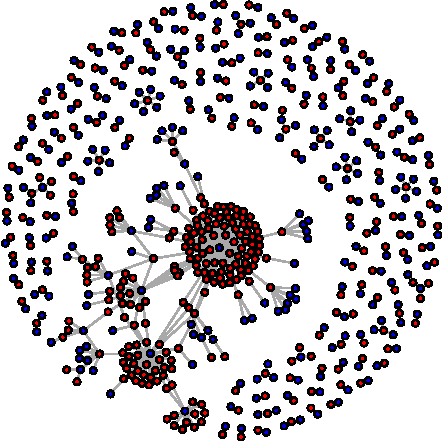
\includegraphics[keepaspectratio]{DataScience_files/figure-latex/unnamed-chunk-5-1.pdf}}
todo \ldots{} Insights aus dem Plot ziehen

Da die Datengrundlage nicht in einem igraph-Objekt vorliegt und
ungerichtet ist, ist es notwendig Knoten, Kanten sowie relevante
Attribute wie beispielsweise Gewichtungen zu definieren, um überhaupt
Netzwerkvisualisierungen in R durchführen zu können. Doch dazu mehr im
nächsten Kapitel.

\newpage

\section{Analysestrategie}\label{analysestrategie}

\begin{enumerate}
\def\labelenumi{\arabic{enumi}.}
\tightlist
\item
  Geografisches Netzwerk
\end{enumerate}

Das Ziel besteht in der Erstellung eines Netzwerkes, welches auf der
räumlichen Nähe von Unternehmen basiert. Auf diese Weise soll untersucht
werden, inwiefern regional bedingte Faktoren die Gehälter beeinflussen.
Die Bildung von Kanten erfolgt nach dem Kriterium der räumlichen Nähe.
Dabei werden Unternehmen, die im gleichen Ort angesiedelt sind, durch
Kanten verbunden.

\begin{enumerate}
\def\labelenumi{\arabic{enumi}.}
\setcounter{enumi}{1}
\tightlist
\item
  Wettbewerbsnetzwerk
\end{enumerate}

Die vorliegende Untersuchung zielt darauf ab, den Einfluss des
Wettbewerbs auf die Gestaltung von Gehaltsstrukturen zu analysieren.
Dazu werden die Beziehungen zwischen konkurrierenden Unternehmen als
Netzwerk dargestellt. Die Bildung von Kanten durch Konkurrenzen erfolgt
wie folgt: Die in der Spalte ``Competitors'' gelisteten Unternehmen
werden als Knoten verbunden. In Bezug auf die Gewichtung sind
verschiedene Optionen denkbar. Beispielsweise könnte die direkte
Konkurrenz mit dem Wert ``1'' und die indirekte Konkurrenz mit dem Wert
``0,5'' bewertet werden. Dabei würde die indirekte Konkurrenz eine
Branche umfassen, in der das Unternehmen zwar nicht als direkter
Konkurrent aufgeführt ist, jedoch potenziell in Konkurrenz stehen
könnte. Im Rahmen der Netzwerkmetriken erfolgt eine Analyse der
folgenden Aspekte: Im Rahmen der Analyse von hierarchischen Beziehungen
und unterschiedlichen Zentralitäten erfolgt eine Untersuchung der
Wichtigkeit eines Unternehmens im Wettbewerbsnetzwerk sowie der
Gehaltshöhen in Relation zur Konkurrenz.

\begin{enumerate}
\def\labelenumi{\arabic{enumi}.}
\setcounter{enumi}{2}
\tightlist
\item
  Vergleich der Gehälter innerhalb der Netzwerke
\end{enumerate}

Im Rahmen der Analyse werden die Gehälter innerhalb der beiden Netzwerke
miteinander verglichen. Ziel ist die Identifikation von Unternehmen, die
zentral in einem der beiden Netzwerke liegen, und solchen, die am Rand
oder isoliert sind, um festzustellen, ob die zentralen Unternehmen
höhere Gehälter anbieten. Zur Durchführung des Gehaltsvergleichs werden
Korrelationen zwischen dem Gehalt und verschiedenen Zentralitätsmaßen
innerhalb der geografischen und wettbewerbsbezogenen Netzwerke
herangezogen. Darüber hinaus werden Cluster-Analysen durchgeführt, um
Unternehmen, die geografisch und wettbewerbsbedingt vernetzt sind,
miteinander zu vergleichen.

\begin{enumerate}
\def\labelenumi{\arabic{enumi}.}
\setcounter{enumi}{3}
\tightlist
\item
  Zusammenführung und Vergleich der Netzwerke
\end{enumerate}

Im Rahmen der Zusammenführung und des Vergleichs der Netzwerke erfolgt
eine Gegenüberstellung der jeweiligen Strukturen, um etwaige
Gemeinsamkeiten und Unterschiede zu identifizieren. Das Ziel dieser
Untersuchung besteht in der Analyse der Interaktion beider Netzwerke
sowie der Identifikation von Regionen, in denen eine besonders hohe
Gehaltskonkurrenz zu beobachten ist. Im Rahmen des Vergleichs der
Netzwerke hinsichtlich der Gehälter und des Wettbewerbs erfolgt zunächst
eine Gegenüberstellung der Gehaltsverteilung in sogenannten
``Hotspot-Regionen'' und geografisch isolierten Regionen. Darüber hinaus
werden gemeinsame Unternehmen in beiden Netzwerken sowie die
Gehaltsstrukturen innerhalb der Überschneidungsbereiche analysiert.

\newpage

\section{Analyse}\label{analyse}

\subsection{Datenbereinigung}\label{datenbereinigung}

\subsubsection{Bereinigung für die geografische
Analyse}\label{bereinigung-fuxfcr-die-geografische-analyse}

Bei der Durchsicht des Datensatzes viel auf, dass die Spalten ``Same
State'' und ``job\_state'' von der Logik her ähnlich sind. Dies soll nun
näher unterucht werden, um spätere Fehler vorzubeugen, vor allem bei den
geografischen Netzwerken vorzubeugen.

\begin{Shaded}
\begin{Highlighting}[]
\CommentTok{\# Auswahl der "State" und "job\_state" Spalten}
\NormalTok{selected\_data }\OtherTok{\textless{}{-}}\NormalTok{ data }\SpecialCharTok{\%\textgreater{}\%}
  \FunctionTok{select}\NormalTok{(State, job\_state)}

\CommentTok{\# Heading der ausgewählten Spalten}
\FunctionTok{head}\NormalTok{(selected\_data, }\DecValTok{15}\NormalTok{)}
\end{Highlighting}
\end{Shaded}

\begin{verbatim}
## # A tibble: 15 x 2
##    State job_state
##    <chr> <chr>    
##  1 NM    NM       
##  2 MD    MD       
##  3 FL    FL       
##  4 WA    WA       
##  5 NY    NY       
##  6 TX    TX       
##  7 MD    MD       
##  8 CA    CA       
##  9 NY    NY       
## 10 NY    NY       
## 11 CA    CA       
## 12 VA    VA       
## 13 TX    TX       
## 14 WA    WA       
## 15 MA    MA
\end{verbatim}

Sieht so aus, als wäre beide Spalten identisch. Dies soll jedoch zur
Probe gestellt werden:

\begin{Shaded}
\begin{Highlighting}[]
\ControlFlowTok{if}\NormalTok{ (}\FunctionTok{all}\NormalTok{(selected\_data}\SpecialCharTok{$}\NormalTok{State }\SpecialCharTok{==}\NormalTok{ selected\_data}\SpecialCharTok{$}\NormalTok{job\_state, }\AttributeTok{na.rm =} \ConstantTok{TRUE}\NormalTok{)) \{}
  \FunctionTok{print}\NormalTok{(}\StringTok{"Alle Werte in \textquotesingle{}State\textquotesingle{} und \textquotesingle{}job\_state\textquotesingle{} sind identisch."}\NormalTok{)}
\NormalTok{\} }\ControlFlowTok{else}\NormalTok{ \{}
  \FunctionTok{print}\NormalTok{(}\StringTok{"Es gibt Unterschiede zwischen \textquotesingle{}State\textquotesingle{} und \textquotesingle{}job\_state\textquotesingle{}."}\NormalTok{)}
\NormalTok{\}}
\end{Highlighting}
\end{Shaded}

\begin{verbatim}
## [1] "Es gibt Unterschiede zwischen 'State' und 'job_state'."
\end{verbatim}

Jedoch trügt der Schein, da es Unterschiede gibt.

\begin{Shaded}
\begin{Highlighting}[]
\CommentTok{\# Auswahl der Zeilen, in denen "State" und "job\_state" unterschiedlich sind}
\NormalTok{different\_states }\OtherTok{\textless{}{-}}\NormalTok{ selected\_data }\SpecialCharTok{\%\textgreater{}\%}
  \FunctionTok{filter}\NormalTok{(State }\SpecialCharTok{!=}\NormalTok{ job\_state)}

\FunctionTok{print}\NormalTok{(different\_states, }\AttributeTok{n =} \ConstantTok{Inf}\NormalTok{)}
\end{Highlighting}
\end{Shaded}

\begin{verbatim}
## # A tibble: 1 x 2
##   State       job_state
##   <chr>       <chr>    
## 1 Los Angeles CA
\end{verbatim}

Es fällt auf, das LA und Los Angeles nicht einheitlich verwendet werden.
Außerdem ist Los Angeles kein eigener Bundesstaat, sonder ein Teil von
Kalifornien(CA). Dies soll nun korrigiert werden.

Außerdem sollte bei weieren Vorgehen beachtet werden, dass Werte wie
``Na'' oder ``-1'' vor den Analysen entfernt werden sollten.

\begin{Shaded}
\begin{Highlighting}[]
\CommentTok{\# Ersetzen von "Los Angeles" durch "LA" und "LA" durch "CA"}
\NormalTok{data }\OtherTok{\textless{}{-}}\NormalTok{ data }\SpecialCharTok{\%\textgreater{}\%}
  \FunctionTok{mutate}\NormalTok{(}\AttributeTok{State =} \FunctionTok{ifelse}\NormalTok{(State }\SpecialCharTok{==} \StringTok{"Los Angeles"}\NormalTok{, }\StringTok{"LA"}\NormalTok{, State),}
         \AttributeTok{job\_state =} \FunctionTok{ifelse}\NormalTok{(job\_state }\SpecialCharTok{==} \StringTok{"Los Angeles"}\NormalTok{, }\StringTok{"LA"}\NormalTok{, job\_state))}

\NormalTok{data }\OtherTok{\textless{}{-}}\NormalTok{ data }\SpecialCharTok{\%\textgreater{}\%}
  \FunctionTok{mutate}\NormalTok{(}\AttributeTok{State =} \FunctionTok{ifelse}\NormalTok{(State }\SpecialCharTok{==} \StringTok{"LA"}\NormalTok{, }\StringTok{"CA"}\NormalTok{, State),}
         \AttributeTok{job\_state =} \FunctionTok{ifelse}\NormalTok{(job\_state }\SpecialCharTok{==} \StringTok{"LA"}\NormalTok{, }\StringTok{"CA"}\NormalTok{, job\_state))}

\CommentTok{\# Erneute Überprüfung}
\NormalTok{selected\_data }\OtherTok{\textless{}{-}}\NormalTok{ data }\SpecialCharTok{\%\textgreater{}\%}
  \FunctionTok{select}\NormalTok{(State, job\_state)}

\ControlFlowTok{if}\NormalTok{ (}\FunctionTok{all}\NormalTok{(selected\_data}\SpecialCharTok{$}\NormalTok{State }\SpecialCharTok{==}\NormalTok{ selected\_data}\SpecialCharTok{$}\NormalTok{job\_state, }\AttributeTok{na.rm =} \ConstantTok{TRUE}\NormalTok{)) \{}
  \FunctionTok{print}\NormalTok{(}\StringTok{"Alle Werte in \textquotesingle{}State\textquotesingle{} und \textquotesingle{}job\_state\textquotesingle{} sind identisch."}\NormalTok{)}
\NormalTok{\} }\ControlFlowTok{else}\NormalTok{ \{}
  \FunctionTok{print}\NormalTok{(}\StringTok{"Es gibt Unterschiede zwischen \textquotesingle{}State\textquotesingle{} und \textquotesingle{}job\_state\textquotesingle{}."}\NormalTok{)}
\NormalTok{\}}
\end{Highlighting}
\end{Shaded}

\begin{verbatim}
## [1] "Alle Werte in 'State' und 'job_state' sind identisch."
\end{verbatim}

\subsubsection{Überprüfung auf weitere fehlende
Werte}\label{uxfcberpruxfcfung-auf-weitere-fehlende-werte}

\begin{Shaded}
\begin{Highlighting}[]
\CommentTok{\# Überprüfen auf NA{-}Werte}

\NormalTok{na\_counts }\OtherTok{\textless{}{-}} \FunctionTok{colSums}\NormalTok{(}\FunctionTok{is.na}\NormalTok{(data))}
\FunctionTok{print}\NormalTok{(}\StringTok{"Anzahl der NA{-}Werte pro Spalte:"}\NormalTok{)}
\end{Highlighting}
\end{Shaded}

\begin{verbatim}
## [1] "Anzahl der NA-Werte pro Spalte:"
\end{verbatim}

\begin{Shaded}
\begin{Highlighting}[]
\FunctionTok{print}\NormalTok{(na\_counts)}
\end{Highlighting}
\end{Shaded}

\begin{verbatim}
##         Job Title   Salary Estimate   Job Description            Rating 
##                 0                 0                 0                 0 
##      Company Name          Location      Headquarters              Size 
##                 0                 0                 0                 0 
##           Founded Type of ownership          Industry            Sector 
##                 0                 0                 0                 0 
##           Revenue       Competitors        Min_Salary        Max_Salary 
##                 0                 0                 0                 0 
##             State        Same State               Age         Python_yn 
##                 0                 0                 0                 0 
##          R Studio             Spark            AWS_yn          Excel_yn 
##                 0                 0                 0                 0 
##          Job_simp         job_state          desc_len          Num_comp 
##                 0                 0                 0                 0
\end{verbatim}

\begin{Shaded}
\begin{Highlighting}[]
\CommentTok{\# Überprüfen auf {-}1{-}Werte}
\NormalTok{neg\_one\_counts }\OtherTok{\textless{}{-}} \FunctionTok{sapply}\NormalTok{(data, }\ControlFlowTok{function}\NormalTok{(x) }\FunctionTok{sum}\NormalTok{(x }\SpecialCharTok{==} \SpecialCharTok{{-}}\DecValTok{1}\NormalTok{, }\AttributeTok{na.rm =} \ConstantTok{TRUE}\NormalTok{))}
\FunctionTok{print}\NormalTok{(}\StringTok{"Anzahl der {-}1{-}Werte pro Spalte:"}\NormalTok{)}
\end{Highlighting}
\end{Shaded}

\begin{verbatim}
## [1] "Anzahl der -1-Werte pro Spalte:"
\end{verbatim}

\begin{Shaded}
\begin{Highlighting}[]
\FunctionTok{print}\NormalTok{(neg\_one\_counts)}
\end{Highlighting}
\end{Shaded}

\begin{verbatim}
##         Job Title   Salary Estimate   Job Description            Rating 
##                 0                 0                 0                11 
##      Company Name          Location      Headquarters              Size 
##                 0                 0                 1                 1 
##           Founded Type of ownership          Industry            Sector 
##                50                 1                10                10 
##           Revenue       Competitors        Min_Salary        Max_Salary 
##                 1               460                 0                 0 
##             State        Same State               Age         Python_yn 
##                 0                 0                50                 0 
##          R Studio             Spark            AWS_yn          Excel_yn 
##                 0                 0                 0                 0 
##          Job_simp         job_state          desc_len          Num_comp 
##                 0                 0                 0                 0
\end{verbatim}

Es zeigt sich, dass es keine NA-Werte gibt, jedoch einige -1-Werte, die
entfert werden sollten.

\begin{Shaded}
\begin{Highlighting}[]
\CommentTok{\# Entfernen von Zeilen mit {-}1 Werten}
\NormalTok{data }\OtherTok{\textless{}{-}}\NormalTok{ data }\SpecialCharTok{\%\textgreater{}\%}
  \FunctionTok{filter\_all}\NormalTok{(}\FunctionTok{all\_vars}\NormalTok{(. }\SpecialCharTok{!=} \SpecialCharTok{{-}}\DecValTok{1}\NormalTok{))}

\CommentTok{\# Überprüfen auf {-}1{-}Werte nach Entfernung}
\NormalTok{neg\_one\_counts }\OtherTok{\textless{}{-}} \FunctionTok{sapply}\NormalTok{(data, }\ControlFlowTok{function}\NormalTok{(x) }\FunctionTok{sum}\NormalTok{(x }\SpecialCharTok{==} \SpecialCharTok{{-}}\DecValTok{1}\NormalTok{, }\AttributeTok{na.rm =} \ConstantTok{TRUE}\NormalTok{))}
\FunctionTok{print}\NormalTok{(}\StringTok{"Anzahl der {-}1 Werte pro Spalte:"}\NormalTok{)}
\end{Highlighting}
\end{Shaded}

\begin{verbatim}
## [1] "Anzahl der -1 Werte pro Spalte:"
\end{verbatim}

\begin{Shaded}
\begin{Highlighting}[]
\FunctionTok{print}\NormalTok{(neg\_one\_counts)}
\end{Highlighting}
\end{Shaded}

\begin{verbatim}
##         Job Title   Salary Estimate   Job Description            Rating 
##                 0                 0                 0                 0 
##      Company Name          Location      Headquarters              Size 
##                 0                 0                 0                 0 
##           Founded Type of ownership          Industry            Sector 
##                 0                 0                 0                 0 
##           Revenue       Competitors        Min_Salary        Max_Salary 
##                 0                 0                 0                 0 
##             State        Same State               Age         Python_yn 
##                 0                 0                 0                 0 
##          R Studio             Spark            AWS_yn          Excel_yn 
##                 0                 0                 0                 0 
##          Job_simp         job_state          desc_len          Num_comp 
##                 0                 0                 0                 0
\end{verbatim}

\subsubsection{Entfernen irrelevanter
Spalten}\label{entfernen-irrelevanter-spalten}

Basierend auf der Analysestrategie und den geplanten Analysen werden
jetzt noch die Spalten, die nicht für die anfängliche geografische
Analyse und die nachfolgende Wettbewerbsanalyse benötigt werden,
entfernt.

\begin{Shaded}
\begin{Highlighting}[]
\CommentTok{\# Entfernen irrelevanter Spalten}
\CommentTok{\# Job Description, Rating, Headquarters, Size, Founded, Type of ownership, Sector, Revenue und Skills}
\NormalTok{data }\OtherTok{\textless{}{-}}\NormalTok{ data }\SpecialCharTok{\%\textgreater{}\%}
  \FunctionTok{select}\NormalTok{(}\SpecialCharTok{{-}}\FunctionTok{c}\NormalTok{(}\StringTok{\textasciigrave{}}\AttributeTok{Job Description}\StringTok{\textasciigrave{}}\NormalTok{, Rating, Headquarters, Size, Founded,}
            \StringTok{\textasciigrave{}}\AttributeTok{Type of ownership}\StringTok{\textasciigrave{}}\NormalTok{, Sector, Revenue,}
\NormalTok{            Python\_yn, }\StringTok{\textasciigrave{}}\AttributeTok{R Studio}\StringTok{\textasciigrave{}}\NormalTok{, Spark, AWS\_yn, Excel\_yn))}

\CommentTok{\# Ausgeben der noch enthaltenen Spalten}
\FunctionTok{print}\NormalTok{(data }\SpecialCharTok{\%\textgreater{}\%} \FunctionTok{names}\NormalTok{())}
\end{Highlighting}
\end{Shaded}

\begin{verbatim}
##  [1] "Job Title"       "Salary Estimate" "Company Name"    "Location"       
##  [5] "Industry"        "Competitors"     "Min_Salary"      "Max_Salary"     
##  [9] "State"           "Same State"      "Age"             "Job_simp"       
## [13] "job_state"       "desc_len"        "Num_comp"
\end{verbatim}

Nachdem die Bereinigung des Datensatzes abgeschlossen ist, kann mit der
Analyse begonnen werden.

\subsection{Netzwerkbildung und
Visualisierung}\label{netzwerkbildung-und-visualisierung}

\subsubsection{Geografische
Vorbetrachtung}\label{geografische-vorbetrachtung}

Da bei der Betrachtung der Wettbewerbsstruktur die geografische Nähe von
Unternehmen auch eine Rolle spielen kann, soll zunächst ein Netzwerk
erstellt werden, das auf der geografischen Nähe von Unternehmen basiert.
Diese annahme beruht darauf, dass Unternehmen in derselben Region
wahrscheinlich ähnliche Gehälter anbieten. Dies soll Überprüft werden um
diese Arbeit um eine weiter Dimension zu erweitern.

\paragraph{Erstellung eines Geografischen
Netzwerkes}\label{erstellung-eines-geografischen-netzwerkes}

Die Gewichtung erfolgt linear, wobei jeder Standort eine Grundgröße von
3 hat, und für jedes Unternehmen an diesem Standort wird die Größe um
0.5 erhöht. Ab einer Größe von 4.5 wird die Farbe des Standorts
geändert, um die Standorte mit mehreren Unternehmen hervorzuheben.

\begin{Shaded}
\begin{Highlighting}[]
\CommentTok{\# Aus Gründen der Sichtbarkeit, werden bloß Locations mit mehr als einem}
\CommentTok{\# Unternehmen dargestellt.}

\CommentTok{\# Extract relevant columns for geographic visualization}
\NormalTok{edges\_geo }\OtherTok{\textless{}{-}}\NormalTok{ data }\SpecialCharTok{\%\textgreater{}\%}
  \FunctionTok{select}\NormalTok{(}\AttributeTok{Company =} \StringTok{\textasciigrave{}}\AttributeTok{Company Name}\StringTok{\textasciigrave{}}\NormalTok{, }\AttributeTok{Location =} \StringTok{\textasciigrave{}}\AttributeTok{Location}\StringTok{\textasciigrave{}}\NormalTok{) }\SpecialCharTok{\%\textgreater{}\%}
  \FunctionTok{distinct}\NormalTok{()}

\CommentTok{\# Calculate the number of companies per location and filter for locations}
\CommentTok{\# with more than one company}
\NormalTok{location\_counts }\OtherTok{\textless{}{-}}\NormalTok{ edges\_geo }\SpecialCharTok{\%\textgreater{}\%}
  \FunctionTok{group\_by}\NormalTok{(Location) }\SpecialCharTok{\%\textgreater{}\%}
  \FunctionTok{summarise}\NormalTok{(}\AttributeTok{Company\_Count =} \FunctionTok{n}\NormalTok{()) }\SpecialCharTok{\%\textgreater{}\%}
  \FunctionTok{filter}\NormalTok{(Company\_Count }\SpecialCharTok{\textgreater{}} \DecValTok{1}\NormalTok{)  }\CommentTok{\# Keep only locations with more than one company}

\CommentTok{\# Filter edges to include only connections for locations with more than}
\CommentTok{\# one company}
\NormalTok{filtered\_edges }\OtherTok{\textless{}{-}}\NormalTok{ edges\_geo }\SpecialCharTok{\%\textgreater{}\%}
  \FunctionTok{filter}\NormalTok{(Location }\SpecialCharTok{\%in\%}\NormalTok{ location\_counts}\SpecialCharTok{$}\NormalTok{Location)}

\CommentTok{\# Create an igraph object for geographic visualization}
\NormalTok{network\_geo }\OtherTok{\textless{}{-}} \FunctionTok{graph\_from\_data\_frame}\NormalTok{(filtered\_edges, }\AttributeTok{directed =} \ConstantTok{FALSE}\NormalTok{)}

\CommentTok{\# Set vertex colors based on whether the node is a company or a location}
\NormalTok{company\_colors }\OtherTok{\textless{}{-}} \StringTok{"blue"}
\NormalTok{location\_colors }\OtherTok{\textless{}{-}} \FunctionTok{rainbow}\NormalTok{(}\FunctionTok{nrow}\NormalTok{(location\_counts))}

\CommentTok{\# Set vertex size based on the number of companies at each location}
\NormalTok{vertex\_sizes }\OtherTok{\textless{}{-}} \FunctionTok{ifelse}\NormalTok{(}\FunctionTok{V}\NormalTok{(network\_geo)}\SpecialCharTok{$}\NormalTok{name }\SpecialCharTok{\%in\%}\NormalTok{ location\_counts}\SpecialCharTok{$}\NormalTok{Location,}
                       \DecValTok{3} \SpecialCharTok{+}\NormalTok{ location\_counts}\SpecialCharTok{$}\NormalTok{Company\_Count[}
                         \FunctionTok{match}\NormalTok{(}\FunctionTok{V}\NormalTok{(network\_geo)}\SpecialCharTok{$}\NormalTok{name, location\_counts}\SpecialCharTok{$}\NormalTok{Location)}
\NormalTok{                       ] }\SpecialCharTok{*} \FloatTok{0.5}\NormalTok{,  }\CommentTok{\# Linear scaling factor with minimum size 3}
                       \DecValTok{3}\NormalTok{) }\CommentTok{\# Default size for companies}

\CommentTok{\# Assign colors and sizes to vertices}
\FunctionTok{V}\NormalTok{(network\_geo)}\SpecialCharTok{$}\NormalTok{size }\OtherTok{\textless{}{-}}\NormalTok{ vertex\_sizes}
\FunctionTok{V}\NormalTok{(network\_geo)}\SpecialCharTok{$}\NormalTok{color }\OtherTok{\textless{}{-}} \FunctionTok{ifelse}\NormalTok{(}\FunctionTok{V}\NormalTok{(network\_geo)}\SpecialCharTok{$}\NormalTok{name }\SpecialCharTok{\%in\%}\NormalTok{ location\_counts}\SpecialCharTok{$}\NormalTok{Location }\SpecialCharTok{\&}
\NormalTok{                               vertex\_sizes }\SpecialCharTok{\textgreater{}} \FloatTok{4.5}\NormalTok{,}
\NormalTok{                               location\_colors[}\FunctionTok{match}\NormalTok{(}\FunctionTok{V}\NormalTok{(network\_geo)}\SpecialCharTok{$}\NormalTok{name, location\_counts}\SpecialCharTok{$}\NormalTok{Location)],}
                               \StringTok{"grey"}\NormalTok{)}

\CommentTok{\# Plot the network}
\FunctionTok{plot}\NormalTok{(network\_geo,}
     \AttributeTok{vertex.label =} \ConstantTok{NA}\NormalTok{,  }\CommentTok{\# Remove labels from the plot}
     \AttributeTok{vertex.size =} \FunctionTok{V}\NormalTok{(network\_geo)}\SpecialCharTok{$}\NormalTok{size,}
     \AttributeTok{vertex.color =} \FunctionTok{V}\NormalTok{(network\_geo)}\SpecialCharTok{$}\NormalTok{color,}
     \AttributeTok{edge.arrow.size =} \FloatTok{0.3}\NormalTok{,}
     \AttributeTok{layout =}\NormalTok{ layout\_with\_fr,}
\NormalTok{)}

\CommentTok{\# Add legend for locations with size \textgreater{} 4.5}
\NormalTok{location\_indices }\OtherTok{\textless{}{-}} \FunctionTok{match}\NormalTok{(location\_counts}\SpecialCharTok{$}\NormalTok{Location, }\FunctionTok{V}\NormalTok{(network\_geo)}\SpecialCharTok{$}\NormalTok{name)}
\NormalTok{large\_locations }\OtherTok{\textless{}{-}}\NormalTok{ location\_counts}\SpecialCharTok{$}\NormalTok{Location[vertex\_sizes[location\_indices] }\SpecialCharTok{\textgreater{}} \FloatTok{4.5}\NormalTok{]}

\NormalTok{large\_location\_colors }\OtherTok{\textless{}{-}}\NormalTok{ location\_colors[}
  \FunctionTok{match}\NormalTok{(large\_locations, location\_counts}\SpecialCharTok{$}\NormalTok{Location)}
\NormalTok{]}
\FunctionTok{legend}\NormalTok{(}\StringTok{"topright"}\NormalTok{,}
       \AttributeTok{legend =}\NormalTok{ large\_locations,}
       \AttributeTok{col =}\NormalTok{ large\_location\_colors,}
       \AttributeTok{pch =} \DecValTok{19}\NormalTok{,}
       \AttributeTok{title =} \StringTok{"Locations"}\NormalTok{)}
\end{Highlighting}
\end{Shaded}

\pandocbounded{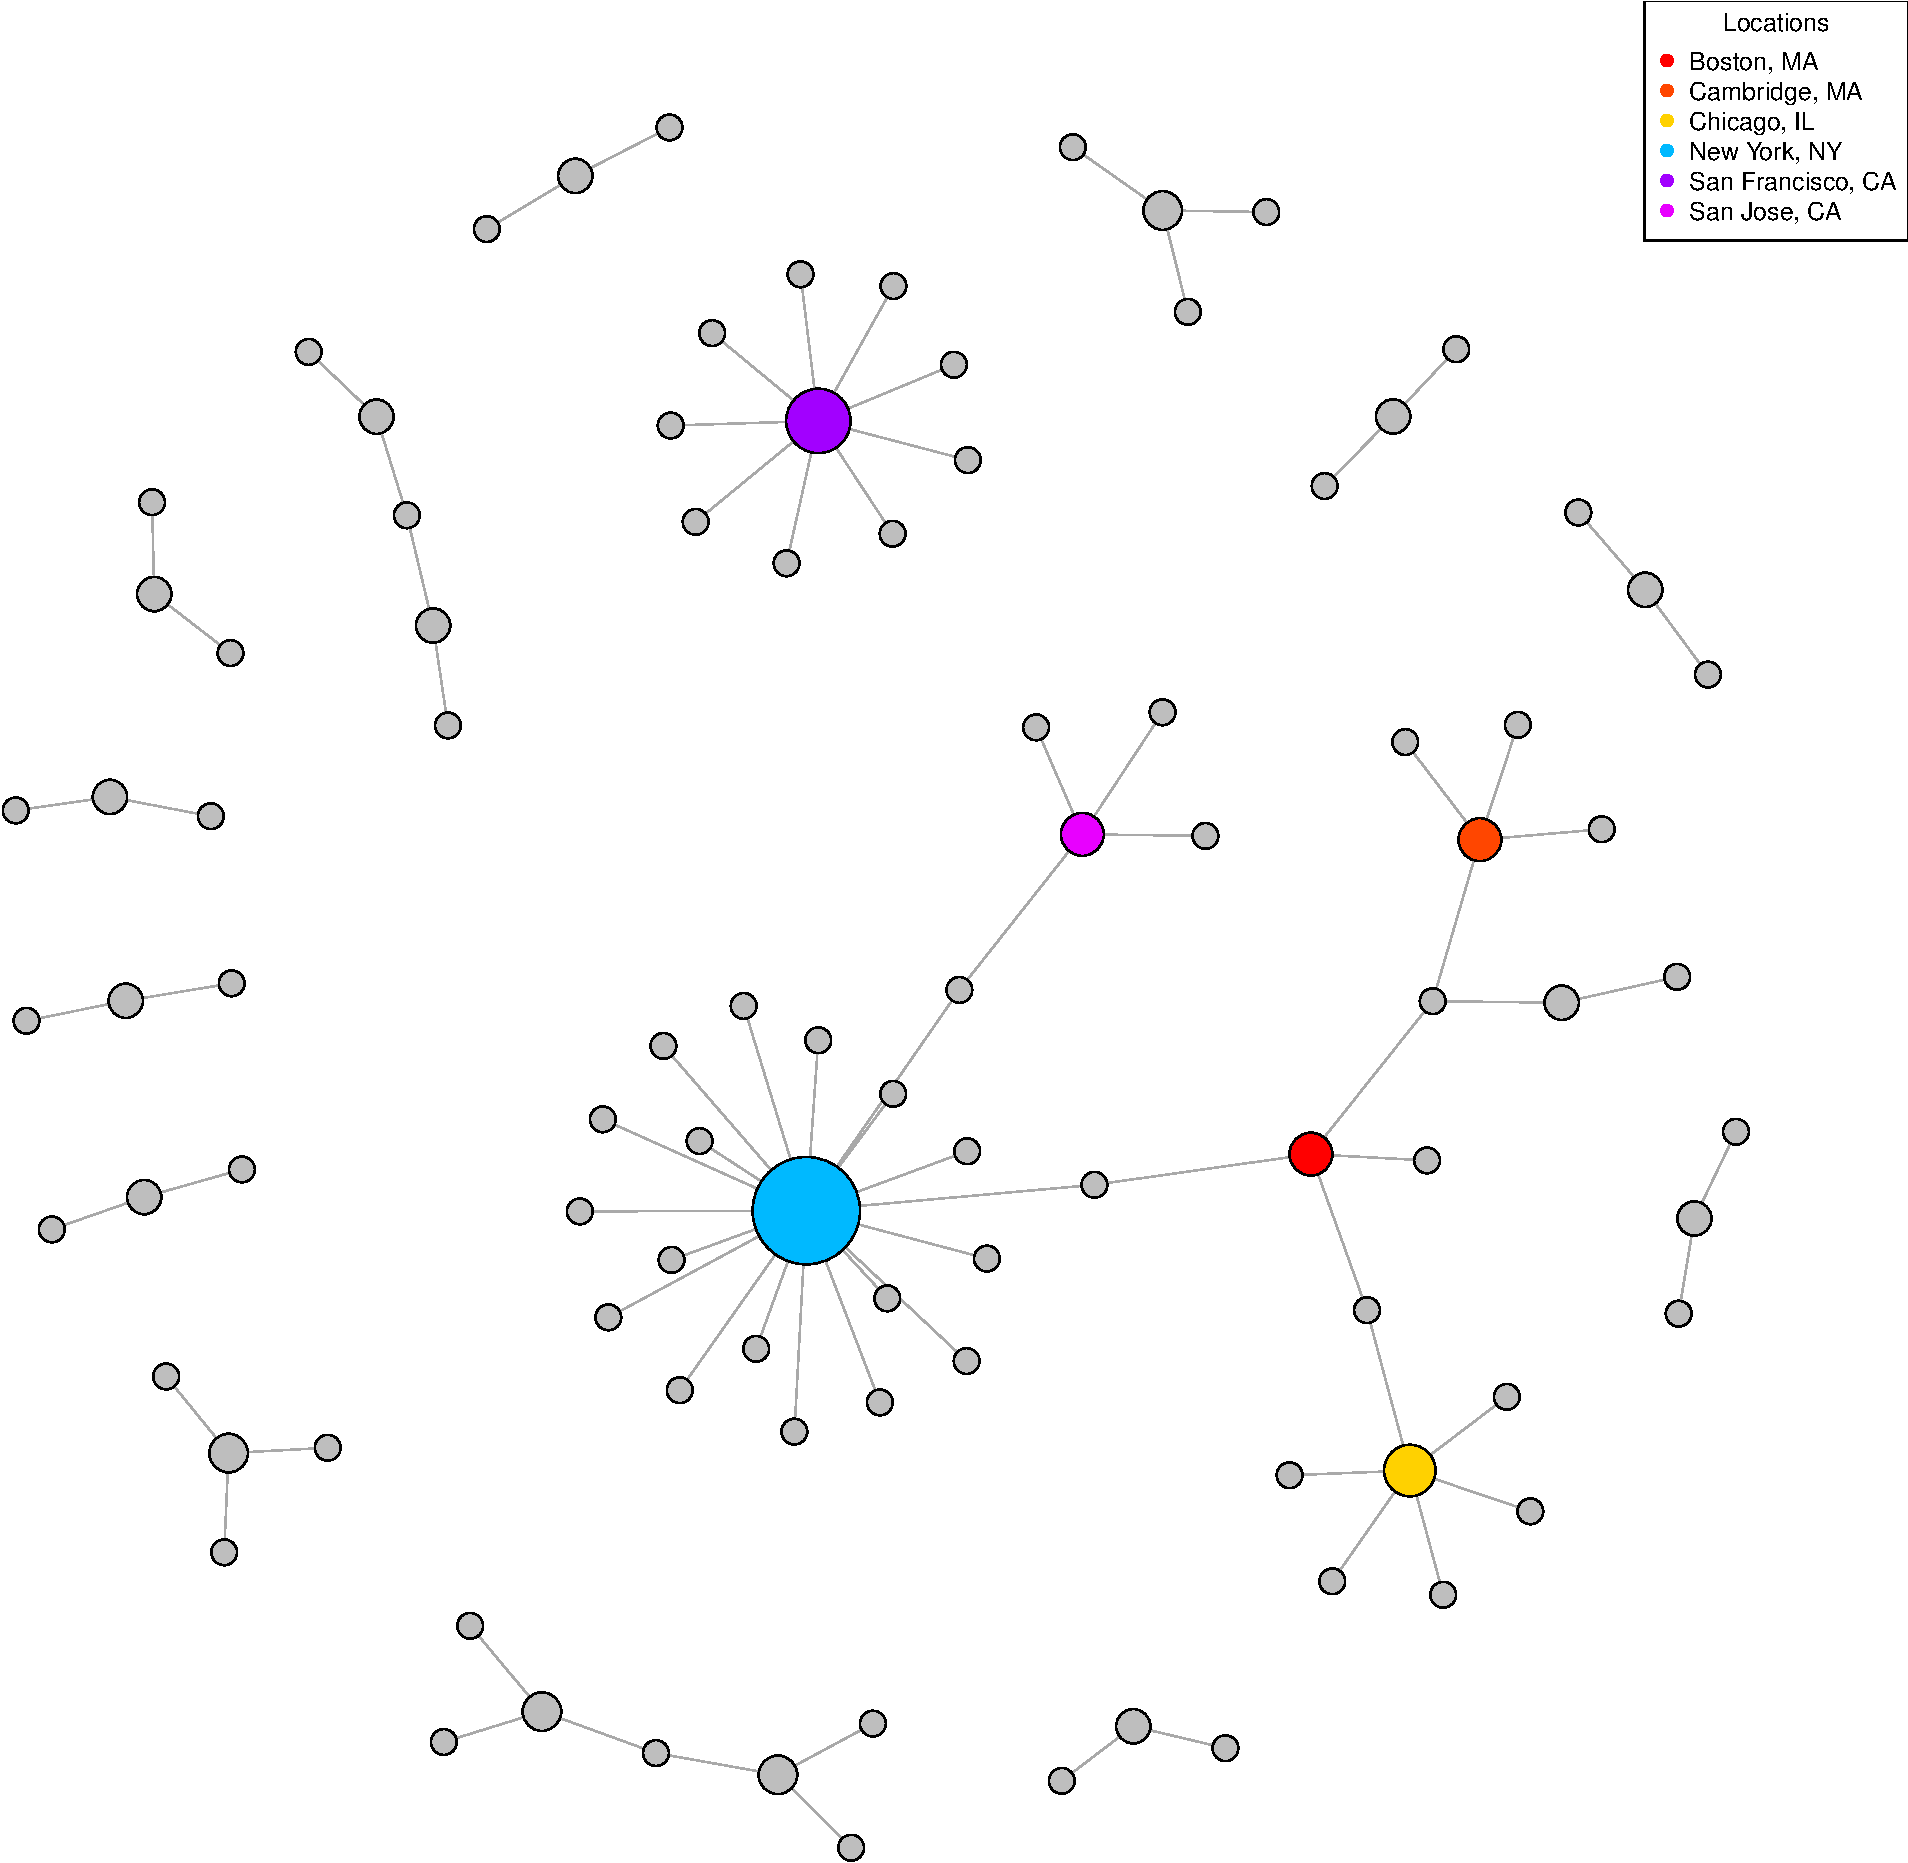
\includegraphics[keepaspectratio]{DataScience_files/figure-latex/unnamed-chunk-13-1.pdf}}

Wie zu erwarten war, sind die meisten Unternehmen Ballungszentren wie
New York, Chicago und San Francisco angesiedelt.

\paragraph{Vergleich der Gehälter zwischen den Hotspot- und den anderen
Regionen}\label{vergleich-der-gehuxe4lter-zwischen-den-hotspot--und-den-anderen-regionen}

\begin{Shaded}
\begin{Highlighting}[]
\CommentTok{\# Ausgabe der farbigen Standorte}
\FunctionTok{print}\NormalTok{(large\_locations)}
\end{Highlighting}
\end{Shaded}

\begin{verbatim}
## [1] "Boston, MA"        "Cambridge, MA"     "Chicago, IL"      
## [4] "New York, NY"      "San Francisco, CA" "San Jose, CA"
\end{verbatim}

\begin{Shaded}
\begin{Highlighting}[]
\CommentTok{\# Filterung der Daten für die Hotspot{-}Regionen}
\NormalTok{data\_hotspots }\OtherTok{\textless{}{-}}\NormalTok{ data }\SpecialCharTok{\%\textgreater{}\%}
  \FunctionTok{filter}\NormalTok{(}\StringTok{\textasciigrave{}}\AttributeTok{Location}\StringTok{\textasciigrave{}} \SpecialCharTok{\%in\%}\NormalTok{ large\_locations)}

\CommentTok{\# Filterung der Daten für die anderen Regionen}
\NormalTok{data\_other }\OtherTok{\textless{}{-}}\NormalTok{ data }\SpecialCharTok{\%\textgreater{}\%}
  \FunctionTok{filter}\NormalTok{(}\SpecialCharTok{!}\StringTok{\textasciigrave{}}\AttributeTok{Location}\StringTok{\textasciigrave{}} \SpecialCharTok{\%in\%}\NormalTok{ large\_locations)}

\CommentTok{\# Durchschnittsgehalt in den Hotspot{-}Regionen}
\NormalTok{avg\_salary\_hotspots }\OtherTok{\textless{}{-}} \FunctionTok{mean}\NormalTok{(data\_hotspots}\SpecialCharTok{$}\StringTok{\textasciigrave{}}\AttributeTok{Salary Estimate}\StringTok{\textasciigrave{}}\NormalTok{, }\AttributeTok{na.rm =} \ConstantTok{TRUE}\NormalTok{)}

\CommentTok{\# Durchschnittsgehalt in den anderen Regionen}
\NormalTok{avg\_salary\_other }\OtherTok{\textless{}{-}} \FunctionTok{mean}\NormalTok{(data\_other}\SpecialCharTok{$}\StringTok{\textasciigrave{}}\AttributeTok{Salary Estimate}\StringTok{\textasciigrave{}}\NormalTok{, }\AttributeTok{na.rm =} \ConstantTok{TRUE}\NormalTok{)}

\CommentTok{\# Erstellung eines Balkendiagramms}
\FunctionTok{ggplot}\NormalTok{(}\AttributeTok{data =} \FunctionTok{data.frame}\NormalTok{(}\AttributeTok{Region =} \FunctionTok{c}\NormalTok{(}\StringTok{"Hotspot"}\NormalTok{, }\StringTok{"Other"}\NormalTok{),}
                         \AttributeTok{Average\_Salary =} \FunctionTok{c}\NormalTok{(avg\_salary\_hotspots,}
\NormalTok{                                            avg\_salary\_other)),}
       \FunctionTok{aes}\NormalTok{(}\AttributeTok{x =}\NormalTok{ Region, }\AttributeTok{y =}\NormalTok{ Average\_Salary, }\AttributeTok{fill =}\NormalTok{ Region)) }\SpecialCharTok{+}
  \FunctionTok{geom\_bar}\NormalTok{(}\AttributeTok{stat =} \StringTok{"identity"}\NormalTok{, }\AttributeTok{width =} \FloatTok{0.4}\NormalTok{) }\SpecialCharTok{+}
  \FunctionTok{scale\_fill\_manual}\NormalTok{(}\AttributeTok{values =} \FunctionTok{c}\NormalTok{(}\StringTok{"Hotspot"} \OtherTok{=} \StringTok{"\#FF5733"}\NormalTok{, }\StringTok{"Other"} \OtherTok{=} \StringTok{"\#33C3FF"}\NormalTok{)) }\SpecialCharTok{+}
  \FunctionTok{labs}\NormalTok{(}\AttributeTok{title =} \StringTok{"Average Salary in Hotspot vs. Other Regions"}\NormalTok{,}
       \AttributeTok{x =} \StringTok{"Region"}\NormalTok{,}
       \AttributeTok{y =} \StringTok{"Average Salary"}\NormalTok{) }\SpecialCharTok{+}
  \FunctionTok{theme\_minimal}\NormalTok{() }\SpecialCharTok{+}
  \FunctionTok{theme}\NormalTok{(}
    \AttributeTok{plot.title =} \FunctionTok{element\_text}\NormalTok{(}\AttributeTok{hjust =} \FloatTok{0.5}\NormalTok{, }\AttributeTok{size =} \DecValTok{14}\NormalTok{, }\AttributeTok{face =} \StringTok{"bold"}\NormalTok{),}
    \AttributeTok{axis.title.x =} \FunctionTok{element\_text}\NormalTok{(}\AttributeTok{size =} \DecValTok{12}\NormalTok{, }\AttributeTok{face =} \StringTok{"bold"}\NormalTok{),}
    \AttributeTok{axis.title.y =} \FunctionTok{element\_text}\NormalTok{(}\AttributeTok{size =} \DecValTok{12}\NormalTok{, }\AttributeTok{face =} \StringTok{"bold"}\NormalTok{),}
    \AttributeTok{axis.text.x =} \FunctionTok{element\_text}\NormalTok{(}\AttributeTok{size =} \DecValTok{12}\NormalTok{),}
    \AttributeTok{axis.text.y =} \FunctionTok{element\_text}\NormalTok{(}\AttributeTok{size =} \DecValTok{12}\NormalTok{),}
    \AttributeTok{legend.position =} \StringTok{"none"}
\NormalTok{  ) }\SpecialCharTok{+}
  \FunctionTok{geom\_text}\NormalTok{(}\FunctionTok{aes}\NormalTok{(}\AttributeTok{label =} \FunctionTok{round}\NormalTok{(Average\_Salary, }\DecValTok{2}\NormalTok{)), }\AttributeTok{vjust =} \SpecialCharTok{{-}}\FloatTok{0.5}\NormalTok{, }\AttributeTok{size =} \DecValTok{4}\NormalTok{)}
\end{Highlighting}
\end{Shaded}

\pandocbounded{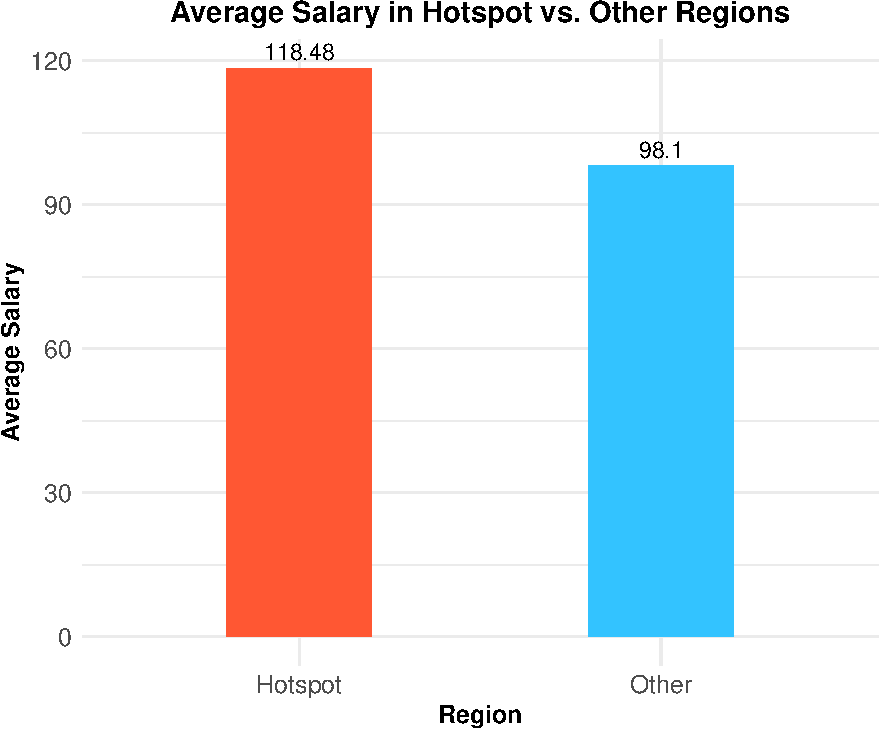
\includegraphics[keepaspectratio]{DataScience_files/figure-latex/unnamed-chunk-14-1.pdf}}

\begin{Shaded}
\begin{Highlighting}[]
\CommentTok{\# Berechnung der Gehaltsunterschiede}
\NormalTok{salary\_diff }\OtherTok{\textless{}{-}}\NormalTok{ avg\_salary\_hotspots }\SpecialCharTok{{-}}\NormalTok{ avg\_salary\_other}

\CommentTok{\# Ausgabe der Gehaltsunterschiede}
\FunctionTok{print}\NormalTok{(}\FunctionTok{paste}\NormalTok{(}\StringTok{"Durchschnittsgehalt in Hotspot{-}Regionen:"}\NormalTok{, avg\_salary\_hotspots))}
\end{Highlighting}
\end{Shaded}

\begin{verbatim}
## [1] "Durchschnittsgehalt in Hotspot-Regionen: 118.475247524752"
\end{verbatim}

\begin{Shaded}
\begin{Highlighting}[]
\FunctionTok{print}\NormalTok{(}\FunctionTok{paste}\NormalTok{(}\StringTok{"Durchschnittsgehalt in anderen Regionen:"}\NormalTok{, avg\_salary\_other))}
\end{Highlighting}
\end{Shaded}

\begin{verbatim}
## [1] "Durchschnittsgehalt in anderen Regionen: 98.1"
\end{verbatim}

\begin{Shaded}
\begin{Highlighting}[]
\FunctionTok{print}\NormalTok{(}\FunctionTok{paste}\NormalTok{(}\StringTok{"Durchschnittlicher Gehaltsunterschied:"}\NormalTok{, salary\_diff))}
\end{Highlighting}
\end{Shaded}

\begin{verbatim}
## [1] "Durchschnittlicher Gehaltsunterschied: 20.3752475247525"
\end{verbatim}

Das Ergebniss zeigt, dass entsprechend der vorher getroffenen Annahme,
die Gehälter in den Hotspot-Regionen im Durchschnitt höher sind als in
anderen Regionen. Dies impliziert eine Korrelation zwischen
geografischer Nähe und Gehaltsniveau.

Deswegen sollen am Ende dieser Arbeit die Ergebnisse der
Wettbewerbsanalyse mit den Ergebnissen der geografischen Analyse
verglichen und in Bezug gesetz werden.

\subsection{Wettbewerbsnetzwerk}\label{wettbewerbsnetzwerk}

In diesem Abschnitt wird mit der eigentlichen Analyse, dem Ziel dieser
Arbeit, der Erstellung einer Wettbewerbsanalyse begonnen.

Zu diesem Zweck wird ein Netzwerk erstellt, das auf den
Wettbewerbsbeziehungen zwischen Unternehmen basiert.

Die Wettbewerbsbeziehungen werden anhand der in der Spalte
``Competitors'' aufgeführten Unternehmen definiert. Die Punkte im
Netzwerk repräsentieren die Unternehmen, während die Kanten die
Wettbewerbsbeziehungen zwischen ihnen darstellen.

Die Gewichtung der Kanten erfolgt wie folgt:

\begin{itemize}
\tightlist
\item
  Direkte Wettbewerber erhalten eine Gewichtung von 1.
\item
  Unternehmen in derselben Branche, jedoch nicht als direkte
  Wettbewerber aufgeführt, erhalten eine Gewichtung von 0.5.
\end{itemize}

Branchenbezogene Wettbewerbsbeziehungen sind in blau dargestellt,
während direkte Wettbewerber in rot hervorgehoben sind.

\begin{Shaded}
\begin{Highlighting}[]
\CommentTok{\# Extrahiere Unternehmen und ihre Wettbewerber}
\NormalTok{edges }\OtherTok{\textless{}{-}}\NormalTok{ data }\SpecialCharTok{\%\textgreater{}\%}
  \FunctionTok{filter}\NormalTok{(}\SpecialCharTok{!}\FunctionTok{is.na}\NormalTok{(Competitors) }\SpecialCharTok{\&}\NormalTok{ Competitors }\SpecialCharTok{!=} \StringTok{"{-}1"}\NormalTok{) }\SpecialCharTok{\%\textgreater{}\%}
  \FunctionTok{separate\_rows}\NormalTok{(Competitors, }\AttributeTok{sep =} \StringTok{", "}\NormalTok{) }\SpecialCharTok{\%\textgreater{}\%}
  \FunctionTok{select}\NormalTok{(}\StringTok{\textasciigrave{}}\AttributeTok{Company Name}\StringTok{\textasciigrave{}}\NormalTok{, Competitors) }\SpecialCharTok{\%\textgreater{}\%}
  \FunctionTok{rename}\NormalTok{(}\AttributeTok{from =} \StringTok{\textasciigrave{}}\AttributeTok{Company Name}\StringTok{\textasciigrave{}}\NormalTok{, }\AttributeTok{to =}\NormalTok{ Competitors) }\SpecialCharTok{\%\textgreater{}\%}
  \FunctionTok{mutate}\NormalTok{(}\AttributeTok{weight =} \DecValTok{1}\NormalTok{)  }\CommentTok{\# Gewichtung für direkte Wettbewerber}

\CommentTok{\# Füge Unternehmen in derselben Branche mit Gewichtung 0.5 hinzu}
\NormalTok{industry\_edges }\OtherTok{\textless{}{-}}\NormalTok{ data }\SpecialCharTok{\%\textgreater{}\%}
  \FunctionTok{filter}\NormalTok{(}\SpecialCharTok{!}\FunctionTok{is.na}\NormalTok{(Industry)) }\SpecialCharTok{\%\textgreater{}\%}
  \FunctionTok{select}\NormalTok{(}\StringTok{\textasciigrave{}}\AttributeTok{Company Name}\StringTok{\textasciigrave{}}\NormalTok{, Industry) }\SpecialCharTok{\%\textgreater{}\%}
  \FunctionTok{inner\_join}\NormalTok{(}
\NormalTok{    data }\SpecialCharTok{\%\textgreater{}\%} \FunctionTok{select}\NormalTok{(}\StringTok{\textasciigrave{}}\AttributeTok{Company Name}\StringTok{\textasciigrave{}}\NormalTok{, Industry),}
    \AttributeTok{by =} \StringTok{"Industry"}\NormalTok{,}
    \AttributeTok{relationship =} \StringTok{"many{-}to{-}many"}
\NormalTok{  ) }\SpecialCharTok{\%\textgreater{}\%}
  \FunctionTok{filter}\NormalTok{(}\StringTok{\textasciigrave{}}\AttributeTok{Company Name.x}\StringTok{\textasciigrave{}} \SpecialCharTok{!=} \StringTok{\textasciigrave{}}\AttributeTok{Company Name.y}\StringTok{\textasciigrave{}}\NormalTok{) }\SpecialCharTok{\%\textgreater{}\%}
  \FunctionTok{select}\NormalTok{(}\AttributeTok{from =} \StringTok{\textasciigrave{}}\AttributeTok{Company Name.x}\StringTok{\textasciigrave{}}\NormalTok{, }\AttributeTok{to =} \StringTok{\textasciigrave{}}\AttributeTok{Company Name.y}\StringTok{\textasciigrave{}}\NormalTok{) }\SpecialCharTok{\%\textgreater{}\%}
  \FunctionTok{mutate}\NormalTok{(}\AttributeTok{weight =} \FloatTok{0.5}\NormalTok{)  }\CommentTok{\# Gewichtung für gleiche Branche}

\CommentTok{\# Kombiniere beide Datensätze}
\NormalTok{all\_edges }\OtherTok{\textless{}{-}} \FunctionTok{bind\_rows}\NormalTok{(edges, industry\_edges)}

\CommentTok{\# Erstelle den Graphen}
\NormalTok{g\_competitors }\OtherTok{\textless{}{-}} \FunctionTok{graph\_from\_data\_frame}\NormalTok{(all\_edges, }\AttributeTok{directed =} \ConstantTok{FALSE}\NormalTok{)}

\CommentTok{\# Entferne mehrere Kanten zwischen denselben Punkten}
\NormalTok{g\_competitors }\OtherTok{\textless{}{-}} \FunctionTok{simplify}\NormalTok{(g\_competitors, }\AttributeTok{remove.multiple =} \ConstantTok{TRUE}\NormalTok{,}
                          \AttributeTok{edge.attr.comb =} \StringTok{"first"}\NormalTok{)}

\CommentTok{\# Setze die Farben der Kanten basierend auf der Gewichtung}
\FunctionTok{E}\NormalTok{(g\_competitors)}\SpecialCharTok{$}\NormalTok{color }\OtherTok{\textless{}{-}} \FunctionTok{ifelse}\NormalTok{(}\FunctionTok{E}\NormalTok{(g\_competitors)}\SpecialCharTok{$}\NormalTok{weight }\SpecialCharTok{==} \DecValTok{1}\NormalTok{, }\StringTok{"red"}\NormalTok{, }\StringTok{"blue"}\NormalTok{)}

\CommentTok{\# Visualisiere das Netzwerk mit kleineren Knoten}
\FunctionTok{plot}\NormalTok{(g\_competitors, }\AttributeTok{vertex.label =} \ConstantTok{NA}\NormalTok{,}
     \AttributeTok{vertex.size =} \DecValTok{2}\NormalTok{,  }\CommentTok{\# Kleinere Knoten}
     \AttributeTok{edge.width =} \FunctionTok{E}\NormalTok{(g\_competitors)}\SpecialCharTok{$}\NormalTok{weight,  }\CommentTok{\# Gewichtung der Kanten}
     \AttributeTok{edge.arrow.size =} \FloatTok{0.5}\NormalTok{,  }\CommentTok{\# Kleinere Pfeile}
     \AttributeTok{main =} \StringTok{"Unternehmensnetzwerk basierend auf Wettbewerbern und Branchen"}\NormalTok{,}
     \AttributeTok{layout =}\NormalTok{ layout\_with\_fr)}

\CommentTok{\# Legende für Kantenfarben}
\FunctionTok{legend}\NormalTok{(}\StringTok{"topright"}\NormalTok{, }\AttributeTok{legend =} \FunctionTok{c}\NormalTok{(}\StringTok{"Direct Competitors"}\NormalTok{, }\StringTok{"Same Industry"}\NormalTok{),}
       \AttributeTok{fill =} \FunctionTok{c}\NormalTok{(}\StringTok{"red"}\NormalTok{, }\StringTok{"blue"}\NormalTok{))}
\end{Highlighting}
\end{Shaded}

\pandocbounded{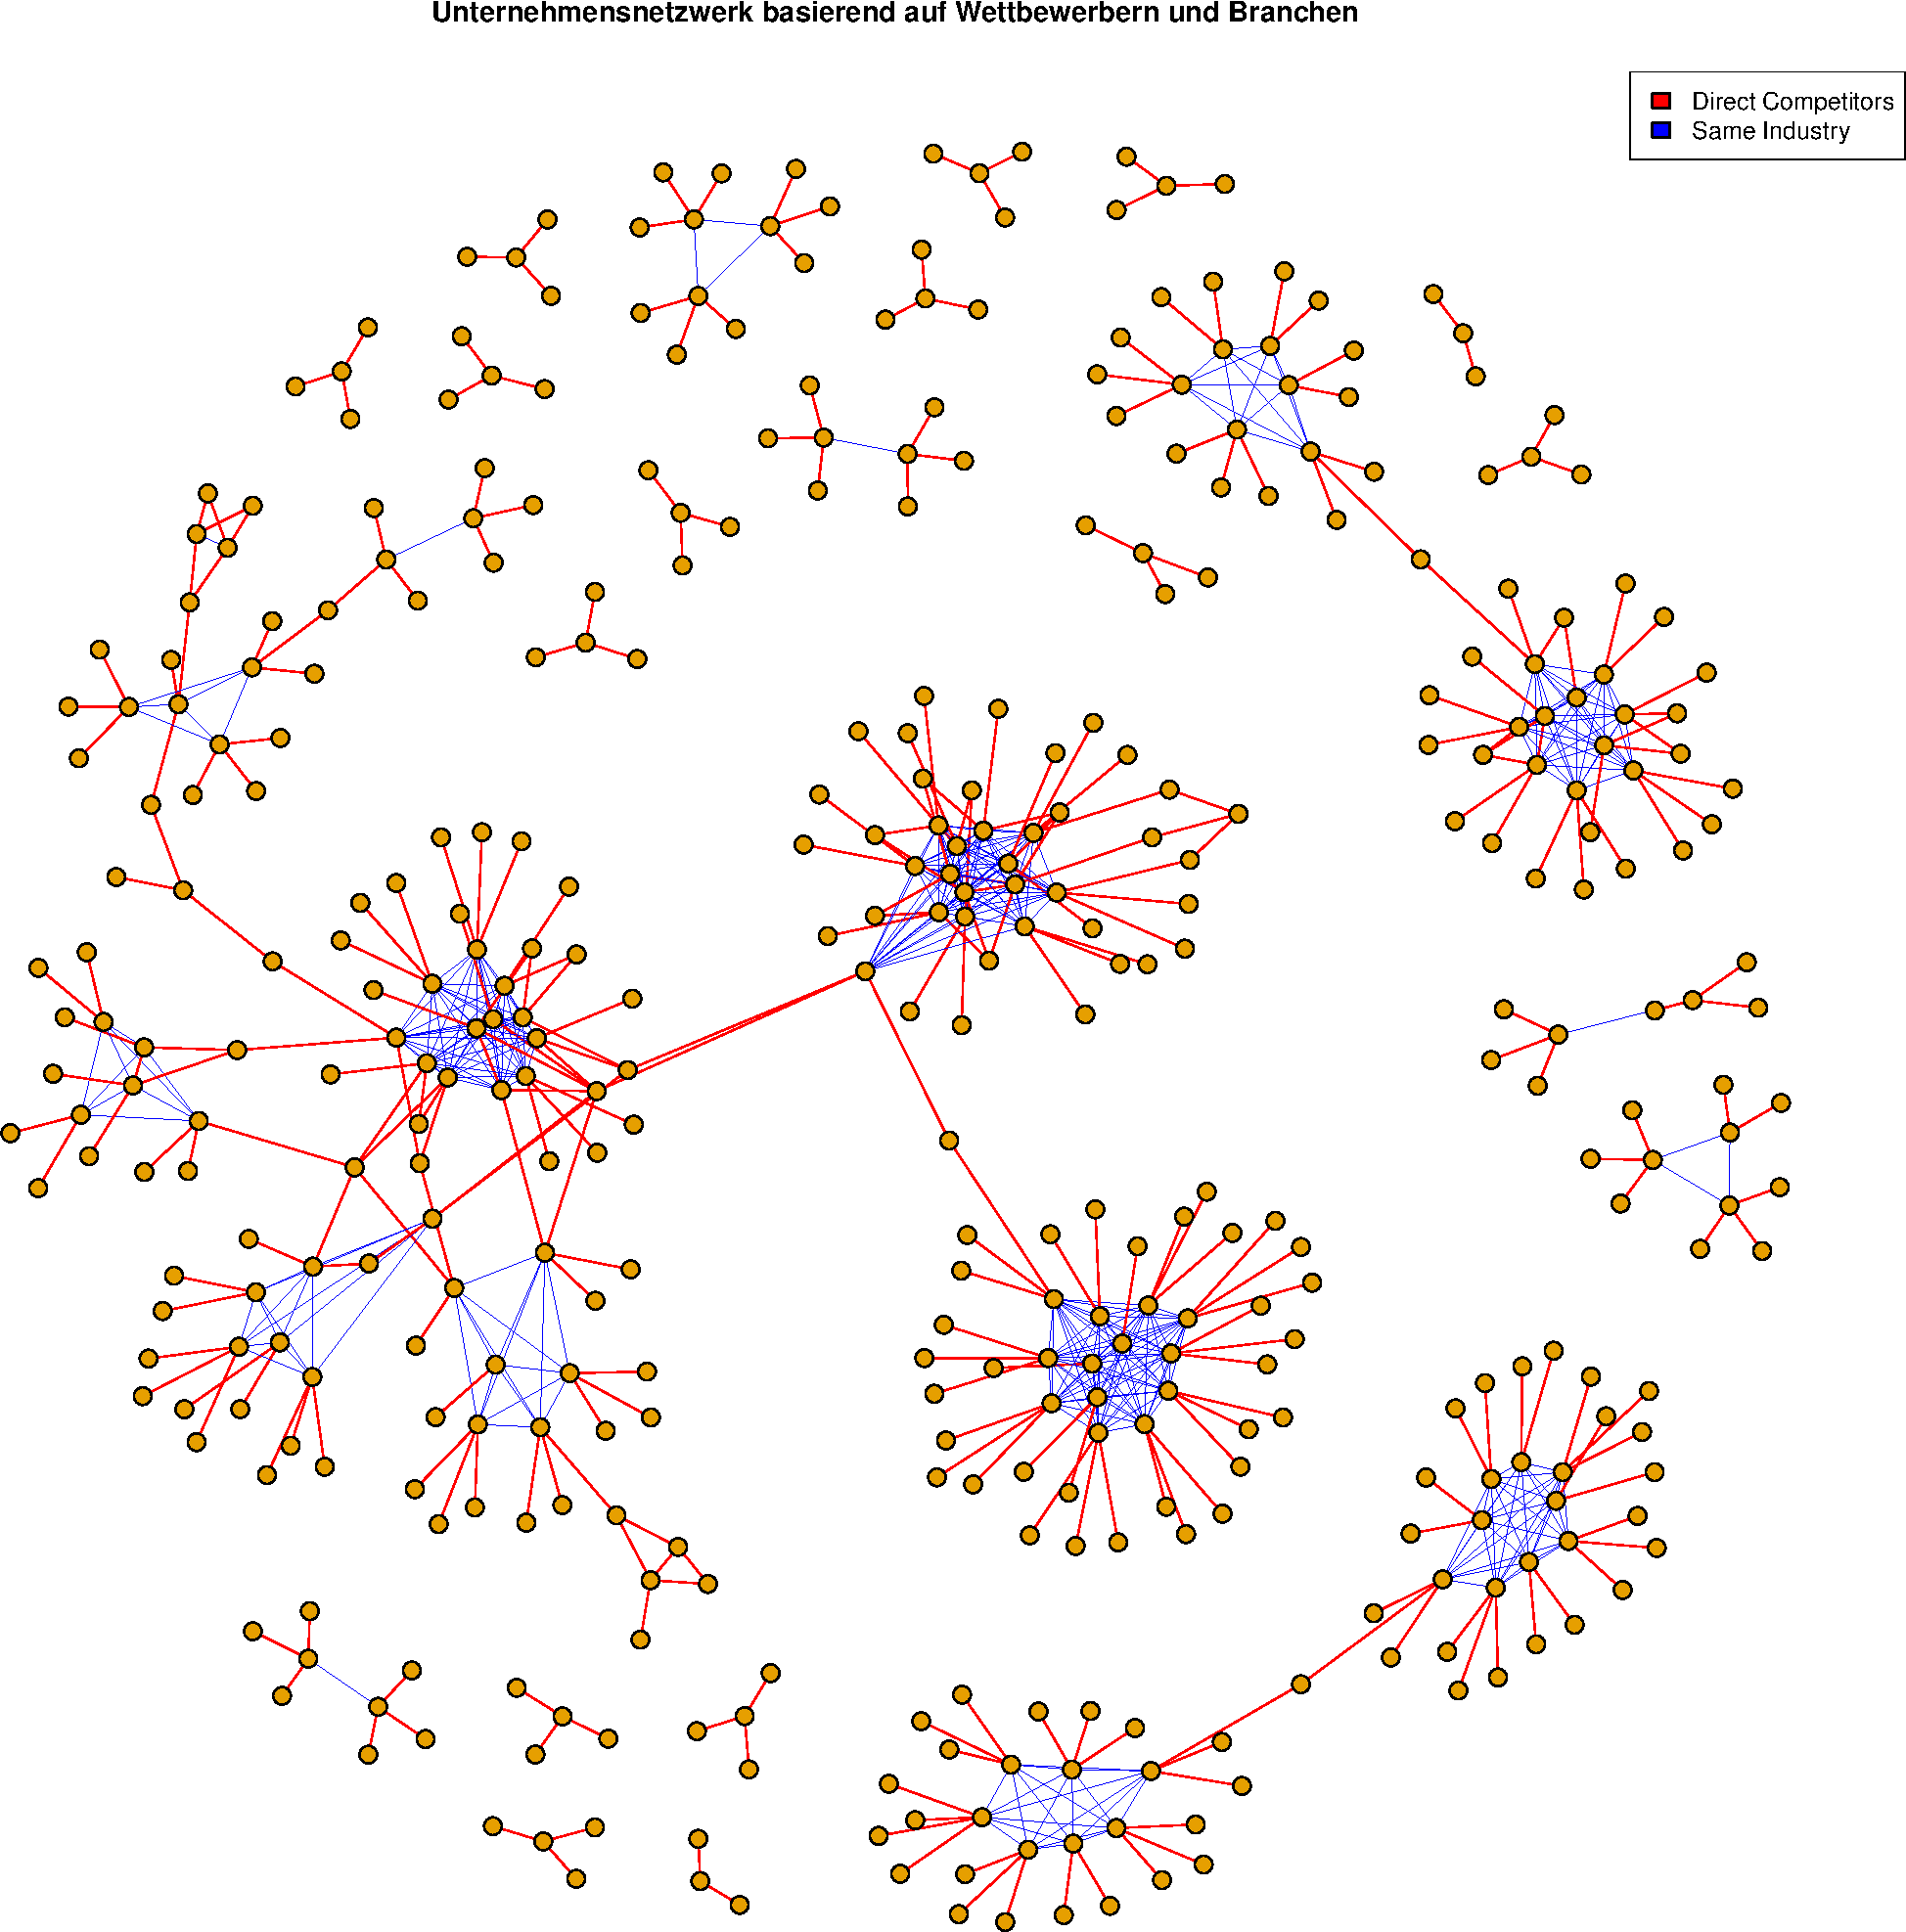
\includegraphics[keepaspectratio]{DataScience_files/figure-latex/unnamed-chunk-16-1.pdf}}
Es lassen sich einige interessante Beobachtungen aus dem Netzwerk
ziehen. Einerseits sind ganz eindeutig Branchencluster zu erkennen, die
auf die Branchenzugehörigkeit der Unternehmen hinweisen.

\begin{Shaded}
\begin{Highlighting}[]
\CommentTok{\# Ausgeben der 10 häufigsten Branchen im Netzwerk}
\NormalTok{top\_industries }\OtherTok{\textless{}{-}}\NormalTok{ data }\SpecialCharTok{\%\textgreater{}\%}
  \FunctionTok{count}\NormalTok{(Industry, }\AttributeTok{sort =} \ConstantTok{TRUE}\NormalTok{) }\SpecialCharTok{\%\textgreater{}\%}
  \FunctionTok{head}\NormalTok{(}\DecValTok{10}\NormalTok{)}

\CommentTok{\# Welche Unternehmen sind in mehreren Branchen vertreten?}
\NormalTok{multi\_industry\_companies }\OtherTok{\textless{}{-}}\NormalTok{ data }\SpecialCharTok{\%\textgreater{}\%}
  \FunctionTok{group\_by}\NormalTok{(}\StringTok{\textasciigrave{}}\AttributeTok{Company Name}\StringTok{\textasciigrave{}}\NormalTok{) }\SpecialCharTok{\%\textgreater{}\%}
  \FunctionTok{summarise}\NormalTok{(}\AttributeTok{Num\_Industries =} \FunctionTok{n\_distinct}\NormalTok{(Industry)) }\SpecialCharTok{\%\textgreater{}\%}
  \FunctionTok{filter}\NormalTok{(Num\_Industries }\SpecialCharTok{\textgreater{}} \DecValTok{1}\NormalTok{) }\SpecialCharTok{\%\textgreater{}\%}
  \FunctionTok{arrange}\NormalTok{(}\FunctionTok{desc}\NormalTok{(Num\_Industries))}

\CommentTok{\# Ausgabe der Unternehmen, die in mehreren Branchen vertreten sind}
\FunctionTok{print}\NormalTok{(multi\_industry\_companies)}
\end{Highlighting}
\end{Shaded}

\begin{verbatim}
## # A tibble: 0 x 2
## # i 2 variables: Company Name <chr>, Num_Industries <int>
\end{verbatim}

Jedoch sind keine Unternehmen in mehreren Branchen vertreten, was darauf
hindeutet, dass die Branchenzugehörigkeit eindeutig ist. Aber es gibt
einige Unternehmen, die mit direkter Konkurrenz die verschiedenen
Branchen verbinden. Dies könnte auf eine Diversifikation der
Geschäftsfelder hindeuten, die eine breitere Wettbewerbsbasis schafft.

Da aber wie oberhalb dargestellt, die Branchenzugehörigkeit eindeutig
ist, und somit die Branchenzugehörigkeit keinen Mehrwert für die Analyse
bietet, wird diese nicht weiter verfolgt.

\subsubsection{Bloß direkte
Wettbewerber}\label{blouxdf-direkte-wettbewerber}

Aus diesem Grund wird das Netzwerk auf direkte Wettbewerber beschränkt,
um die Analyse zu vereinfachen und die Relevanz der
Wettbewerbsbeziehungen zu erhöhen.

\begin{Shaded}
\begin{Highlighting}[]
\CommentTok{\# Extrahiere Unternehmen und ihre Wettbewerber}
\NormalTok{edges }\OtherTok{\textless{}{-}}\NormalTok{ data }\SpecialCharTok{\%\textgreater{}\%}
  \FunctionTok{filter}\NormalTok{(}\SpecialCharTok{!}\FunctionTok{is.na}\NormalTok{(Competitors) }\SpecialCharTok{\&}\NormalTok{ Competitors }\SpecialCharTok{!=} \StringTok{"{-}1"}\NormalTok{) }\SpecialCharTok{\%\textgreater{}\%}
  \FunctionTok{separate\_rows}\NormalTok{(Competitors, }\AttributeTok{sep =} \StringTok{", "}\NormalTok{) }\SpecialCharTok{\%\textgreater{}\%}
  \FunctionTok{select}\NormalTok{(}\StringTok{\textasciigrave{}}\AttributeTok{Company Name}\StringTok{\textasciigrave{}}\NormalTok{, Competitors) }\SpecialCharTok{\%\textgreater{}\%}
  \FunctionTok{rename}\NormalTok{(}\AttributeTok{from =} \StringTok{\textasciigrave{}}\AttributeTok{Company Name}\StringTok{\textasciigrave{}}\NormalTok{, }\AttributeTok{to =}\NormalTok{ Competitors) }\SpecialCharTok{\%\textgreater{}\%}
  \FunctionTok{mutate}\NormalTok{(}\AttributeTok{weight =} \DecValTok{1}\NormalTok{)  }\CommentTok{\# Gewichtung für direkte Wettbewerber}

\CommentTok{\# Summiere die Gewichtungen für mehrere Kanten zwischen denselben Punkten}
\NormalTok{edge\_weights }\OtherTok{\textless{}{-}}\NormalTok{ edges }\SpecialCharTok{\%\textgreater{}\%}
  \FunctionTok{group\_by}\NormalTok{(from, to) }\SpecialCharTok{\%\textgreater{}\%}
  \FunctionTok{summarise}\NormalTok{(}\AttributeTok{weight =} \FunctionTok{sum}\NormalTok{(weight), }\AttributeTok{.groups =} \StringTok{\textquotesingle{}drop\textquotesingle{}}\NormalTok{)}

\CommentTok{\# Erstelle den Graphen nur mit direkten Wettbewerbern}
\NormalTok{g\_direct\_competitors }\OtherTok{\textless{}{-}} \FunctionTok{graph\_from\_data\_frame}\NormalTok{(edge\_weights, }\AttributeTok{directed =} \ConstantTok{FALSE}\NormalTok{)}

\CommentTok{\# Setze die Gewichtungen der Kanten im Graphen}
\FunctionTok{E}\NormalTok{(g\_direct\_competitors)}\SpecialCharTok{$}\NormalTok{weight }\OtherTok{\textless{}{-}}\NormalTok{ edge\_weights}\SpecialCharTok{$}\NormalTok{weight}

\CommentTok{\# Füge die Gehaltsdaten hinzu und berechne das durchschnittliche Gehalt pro Unternehmen}
\NormalTok{salary\_data }\OtherTok{\textless{}{-}}\NormalTok{ data }\SpecialCharTok{\%\textgreater{}\%}
  \FunctionTok{group\_by}\NormalTok{(}\StringTok{\textasciigrave{}}\AttributeTok{Company Name}\StringTok{\textasciigrave{}}\NormalTok{) }\SpecialCharTok{\%\textgreater{}\%}
  \FunctionTok{summarise}\NormalTok{(}\AttributeTok{AverageSalary =} \FunctionTok{mean}\NormalTok{(}\StringTok{\textasciigrave{}}\AttributeTok{Salary Estimate}\StringTok{\textasciigrave{}}\NormalTok{, }\AttributeTok{na.rm =} \ConstantTok{TRUE}\NormalTok{))}

\CommentTok{\# Füge die Gehaltsdaten zu den Knoten des Graphen hinzu}
\FunctionTok{V}\NormalTok{(g\_direct\_competitors)}\SpecialCharTok{$}\NormalTok{salary }\OtherTok{\textless{}{-}}\NormalTok{ salary\_data}\SpecialCharTok{$}\NormalTok{AverageSalary[}\FunctionTok{match}\NormalTok{(}\FunctionTok{V}\NormalTok{(g\_direct\_competitors)}\SpecialCharTok{$}\NormalTok{name, salary\_data}\SpecialCharTok{$}\StringTok{\textasciigrave{}}\AttributeTok{Company Name}\StringTok{\textasciigrave{}}\NormalTok{)]}

\CommentTok{\# Setze die Farben der Knoten basierend auf den Gehältern}
\NormalTok{salary\_quantiles }\OtherTok{\textless{}{-}} \FunctionTok{quantile}\NormalTok{(}\FunctionTok{V}\NormalTok{(g\_direct\_competitors)}\SpecialCharTok{$}\NormalTok{salary, }\AttributeTok{probs =} \FunctionTok{seq}\NormalTok{(}\DecValTok{0}\NormalTok{, }\DecValTok{1}\NormalTok{, }\AttributeTok{length.out =} \DecValTok{6}\NormalTok{), }\AttributeTok{na.rm =} \ConstantTok{TRUE}\NormalTok{)}
\NormalTok{color\_palette }\OtherTok{\textless{}{-}} \FunctionTok{brewer.pal}\NormalTok{(}\DecValTok{5}\NormalTok{, }\StringTok{"YlOrRd"}\NormalTok{)}
\FunctionTok{V}\NormalTok{(g\_direct\_competitors)}\SpecialCharTok{$}\NormalTok{color }\OtherTok{\textless{}{-}} \FunctionTok{cut}\NormalTok{(}\FunctionTok{V}\NormalTok{(g\_direct\_competitors)}\SpecialCharTok{$}\NormalTok{salary, }
                                     \AttributeTok{breaks =}\NormalTok{ salary\_quantiles, }
                                     \AttributeTok{labels =} \ConstantTok{FALSE}\NormalTok{, }
                                     \AttributeTok{include.lowest =} \ConstantTok{TRUE}\NormalTok{)}
\FunctionTok{V}\NormalTok{(g\_direct\_competitors)}\SpecialCharTok{$}\NormalTok{color }\OtherTok{\textless{}{-}}\NormalTok{ color\_palette[}\FunctionTok{V}\NormalTok{(g\_direct\_competitors)}\SpecialCharTok{$}\NormalTok{color]}

\CommentTok{\# Setze die Farben der Kanten basierend auf der Gewichtung}
\FunctionTok{E}\NormalTok{(g\_direct\_competitors)}\SpecialCharTok{$}\NormalTok{color }\OtherTok{\textless{}{-}} \StringTok{"red"}

\CommentTok{\# Visualisiere das Netzwerk mit kleineren Knoten}
\FunctionTok{plot}\NormalTok{(g\_direct\_competitors, }\AttributeTok{vertex.label =} \ConstantTok{NA}\NormalTok{,}
     \AttributeTok{vertex.size =} \DecValTok{3}\NormalTok{,  }\CommentTok{\# Kleinere Knoten}
     \AttributeTok{edge.width =} \DecValTok{1} \SpecialCharTok{*} \FunctionTok{E}\NormalTok{(g\_direct\_competitors)}\SpecialCharTok{$}\NormalTok{weight,  }\CommentTok{\# Reduzierte Gewichtung der Kanten}
     \AttributeTok{edge.arrow.size =} \DecValTok{1}\NormalTok{,}
     \AttributeTok{main =} \StringTok{"Unternehmensnetzwerk basierend auf direkten Wettbewerbern"}\NormalTok{,}
     \AttributeTok{layout =}\NormalTok{ layout\_with\_fr}
\NormalTok{)}

\CommentTok{\# Legende für Knotenfarben}
\FunctionTok{legend}\NormalTok{(}\StringTok{"topright"}\NormalTok{, }\AttributeTok{legend =} \FunctionTok{c}\NormalTok{(}\StringTok{"Lowest Salary"}\NormalTok{, }\StringTok{"Low Salary"}\NormalTok{, }\StringTok{"Medium Salary"}\NormalTok{, }\StringTok{"High Salary"}\NormalTok{, }\StringTok{"Highest Salary"}\NormalTok{),}
       \AttributeTok{fill =}\NormalTok{ color\_palette)}
\end{Highlighting}
\end{Shaded}

\pandocbounded{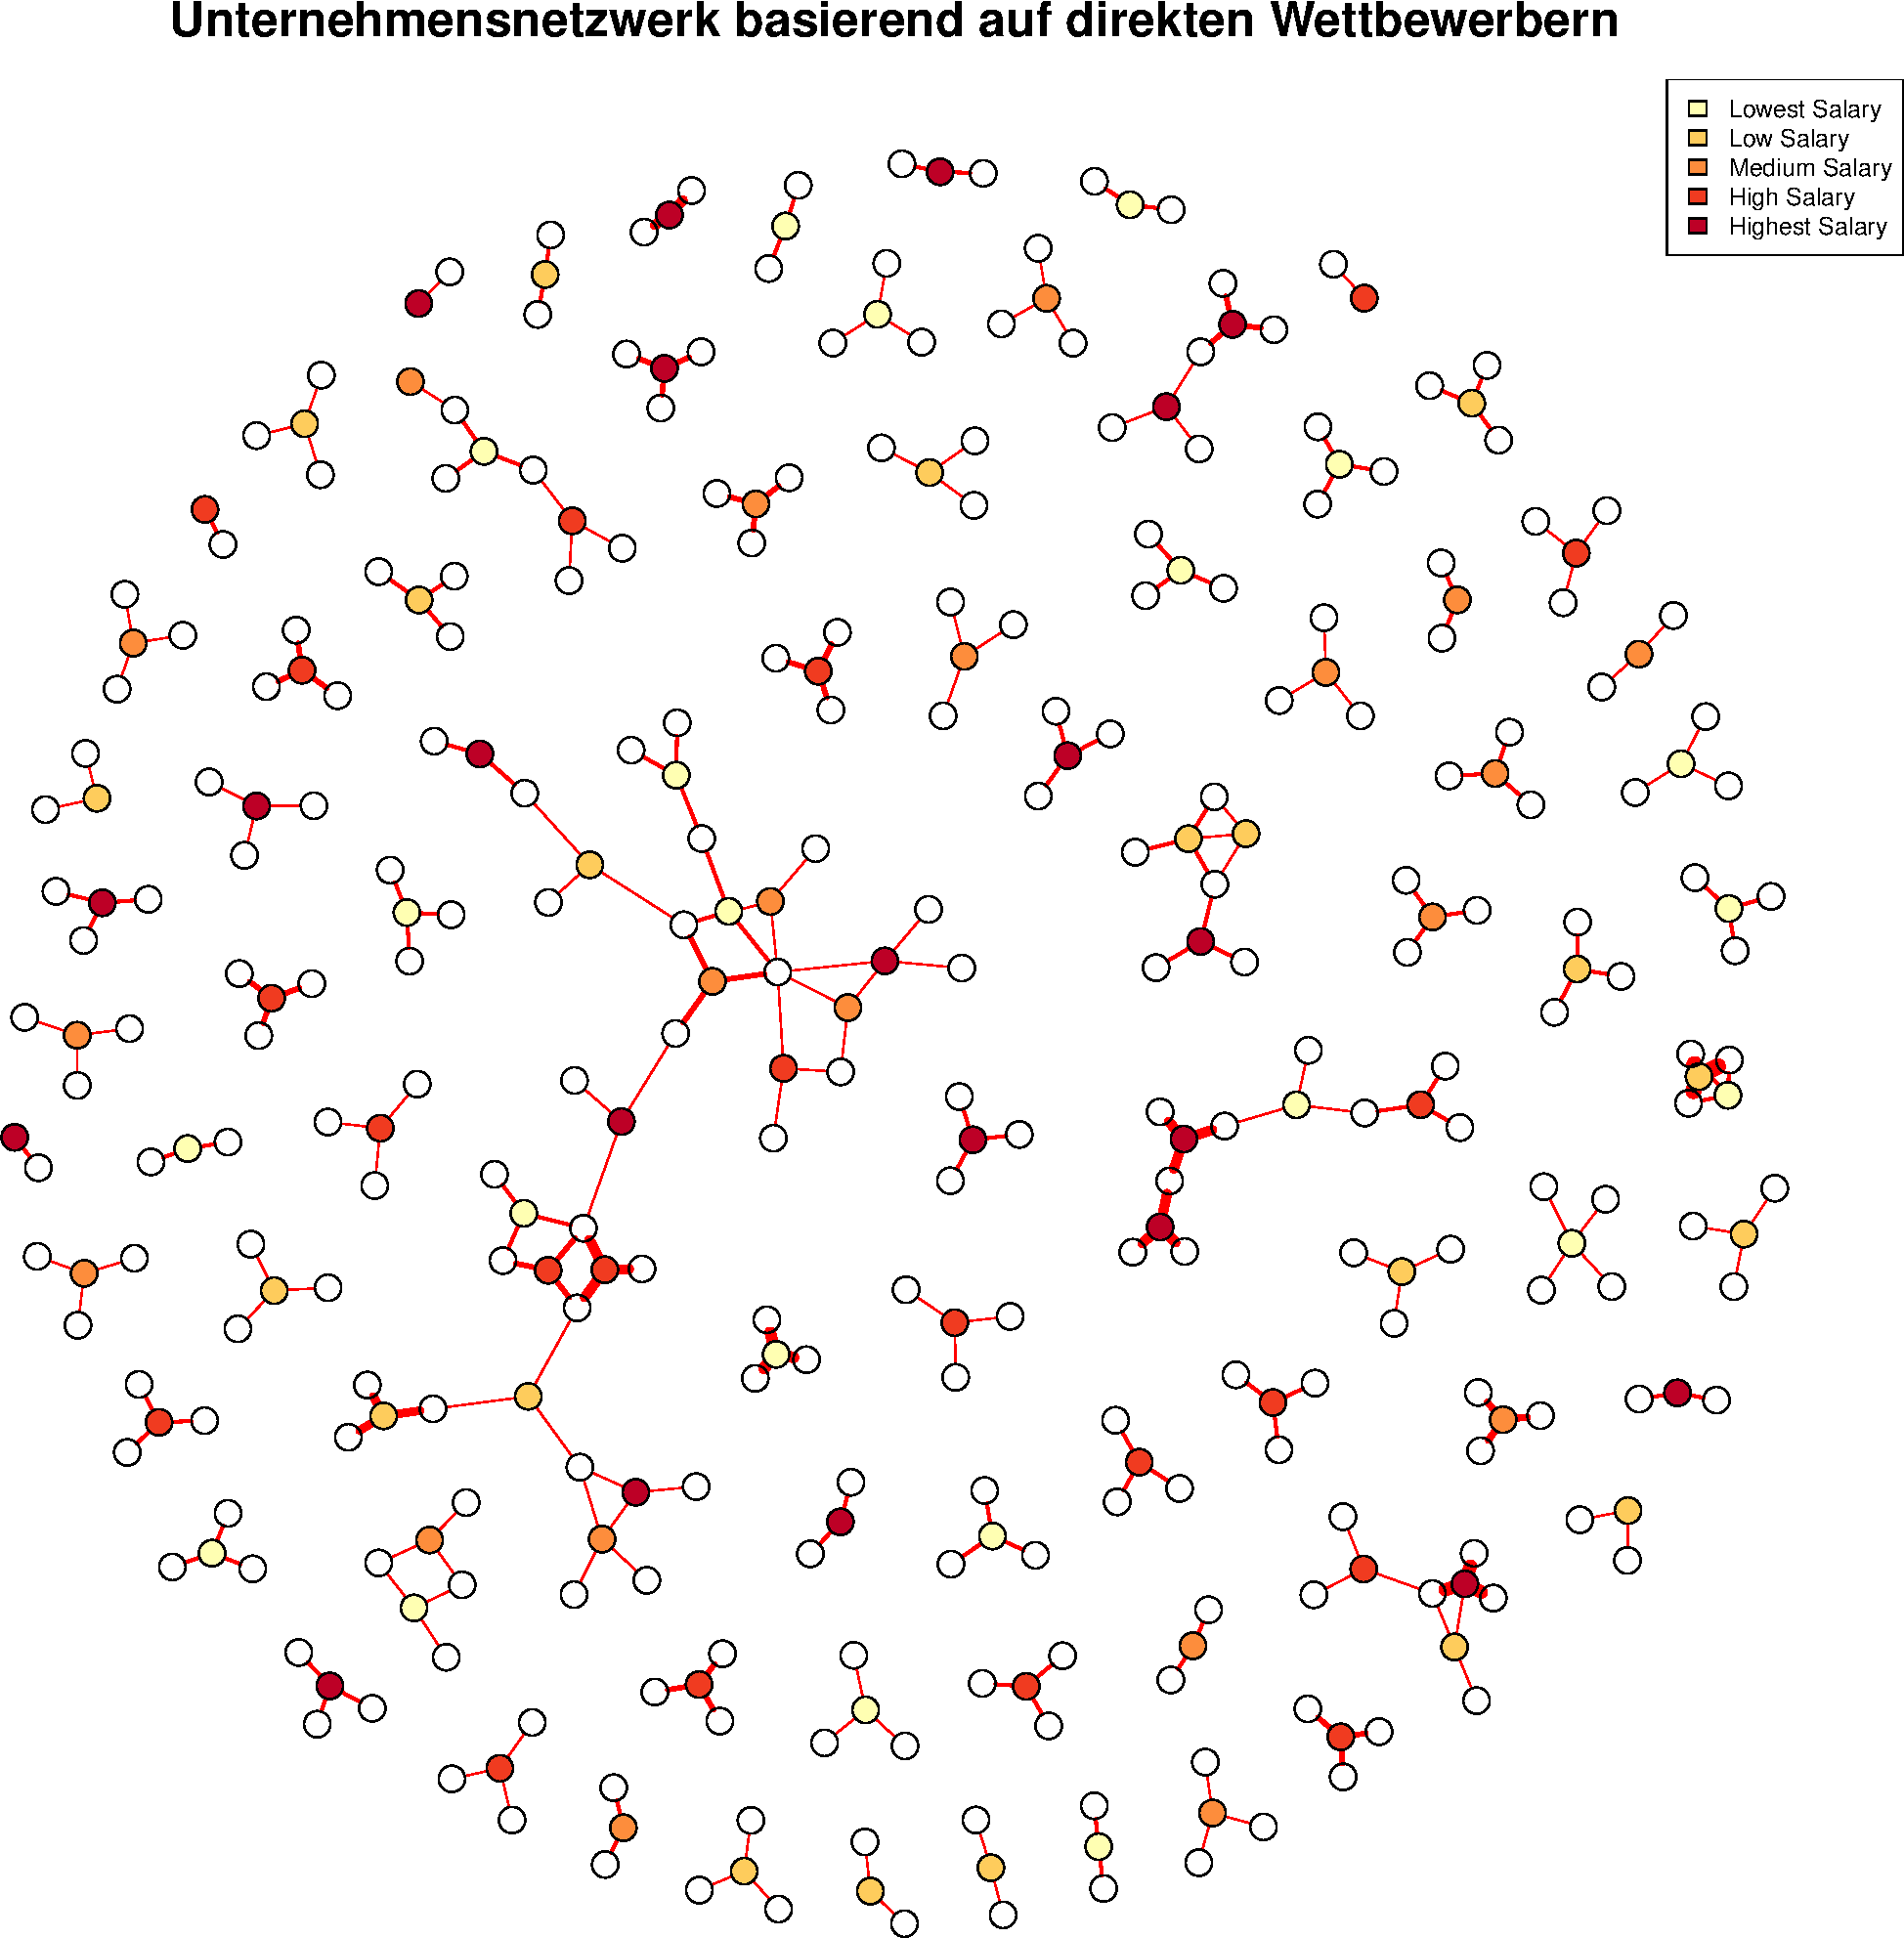
\includegraphics[keepaspectratio]{DataScience_files/figure-latex/unnamed-chunk-18-1.pdf}}

\begin{Shaded}
\begin{Highlighting}[]
\CommentTok{\# Ausgabe der Gehälter der Unternehmen}
\NormalTok{salary\_data }\OtherTok{\textless{}{-}}\NormalTok{ data }\SpecialCharTok{\%\textgreater{}\%}
  \FunctionTok{group\_by}\NormalTok{(}\StringTok{\textasciigrave{}}\AttributeTok{Company Name}\StringTok{\textasciigrave{}}\NormalTok{) }\SpecialCharTok{\%\textgreater{}\%}
  \FunctionTok{summarise}\NormalTok{(}\AttributeTok{AverageSalary =} \FunctionTok{mean}\NormalTok{(}\StringTok{\textasciigrave{}}\AttributeTok{Salary Estimate}\StringTok{\textasciigrave{}}\NormalTok{, }\AttributeTok{na.rm =} \ConstantTok{TRUE}\NormalTok{)) }\SpecialCharTok{\%\textgreater{}\%}
  \FunctionTok{arrange}\NormalTok{(}\FunctionTok{desc}\NormalTok{(AverageSalary))}

\CommentTok{\# Ausgabe aller Unternehmen zusammen mit ihren Gehältern}
\FunctionTok{print}\NormalTok{(salary\_data, }\AttributeTok{n =} \ConstantTok{Inf}\NormalTok{)}
\end{Highlighting}
\end{Shaded}

\begin{verbatim}
## # A tibble: 127 x 2
##     `Company Name`                                      AverageSalary
##     <chr>                                                       <dbl>
##   1 Gallup                                                      238. 
##   2 Credit Sesame                                               205  
##   3 The Climate Corporation                                     194  
##   4 Samsung Research America                                    177  
##   5 Nektar Therapeutics                                         174  
##   6 BioMarin Pharmaceutical                                     168  
##   7 Adobe                                                       162  
##   8 Glassdoor                                                   162  
##   9 Netskope                                                    154. 
##  10 Liberty Mutual Insurance                                    154. 
##  11 Factual                                                     153  
##  12 Visa Inc.                                                   153. 
##  13 Sunovion                                                    151. 
##  14 Sumo Logic                                                  150. 
##  15 Western Digital                                             147. 
##  16 Capgemini                                                   147  
##  17 Tapjoy                                                      147. 
##  18 Mitsubishi Electric Research Labs                           144. 
##  19 1904labs                                                    144. 
##  20 <intent>                                                    140  
##  21 Demandbase                                                  139. 
##  22 Walmart                                                     139  
##  23 Red Ventures                                                134  
##  24 Takeda Pharmaceuticals                                      132. 
##  25 Johns Hopkins University Applied Physics Laboratory         130  
##  26 CBS Interactive                                             128  
##  27 Novetta                                                     128. 
##  28 Information Builders                                        125  
##  29 AstraZeneca                                                 124. 
##  30 TriNet                                                      124. 
##  31 Swiss Re                                                    123  
##  32 L.A. Care Health Plan                                       120. 
##  33 Equity Residential                                          118. 
##  34 PennyMac                                                    117. 
##  35 Affinity Solutions                                          114. 
##  36 Pactera                                                     114. 
##  37 Genesys                                                     112. 
##  38 New England Biolabs                                         112. 
##  39 IQVIA                                                       112. 
##  40 Assurant                                                    110. 
##  41 GNY Insurance Companies                                     110. 
##  42 The Integer Group                                           110  
##  43 The Buffalo Group                                           108. 
##  44 Echo Global Logistics                                       108. 
##  45 Johns Hopkins Health Care                                   108. 
##  46 Mentor Graphics                                             107  
##  47 NCSOFT                                                      106. 
##  48 Porch                                                       106. 
##  49 Medidata Solutions                                          105  
##  50 PA Consulting                                               104  
##  51 Maximus Real Estate Partners                                104. 
##  52 Blueprint Medicines                                         102  
##  53 Genworth                                                    102  
##  54 Blue Cross & Blue Shield of Rhode Island                    100  
##  55 Centro                                                      100  
##  56 PatientPoint                                                100  
##  57 Plymouth Rock Assurance                                      98.5
##  58 Carmeuse                                                     98  
##  59 Pilot Flying J Travel Centers LLC                            98  
##  60 Eventbrite                                                   97.7
##  61 Strategic Financial Solutions                                97.5
##  62 comScore                                                     96.5
##  63 CapTech                                                      95.5
##  64 CyrusOne                                                     95  
##  65 Object Partners                                              95  
##  66 Remedy BPCI Partners, LLC.                                   95  
##  67 Exelixis                                                     93.8
##  68 23andMe                                                      92  
##  69 L&T Infotech                                                 90  
##  70 Lockheed Martin                                              89  
##  71 Productive Edge                                              88.8
##  72 Sauce Labs                                                   88  
##  73 Fivestars                                                    87.5
##  74 GSK                                                          87.5
##  75 Moda Operandi                                                87.5
##  76 Trilogy Ed                                                   87.5
##  77 PNNL                                                         87.0
##  78 AVANADE                                                      87  
##  79 Biz2Credit Inc                                               87  
##  80 Mteq                                                         87  
##  81 Centauri                                                     86.5
##  82 Esri                                                         85.8
##  83 Rapid Response Monitoring                                    85.5
##  84 DICK'S Sporting Goods - Corporate                            85  
##  85 First Command Financial Services, Inc.                       85  
##  86 ICW Group                                                    83  
##  87 Edgewell Personal Care                                       82.5
##  88 MITRE                                                        82.1
##  89 Pharmavite                                                   81.5
##  90 General Dynamics Information Technology                      81.2
##  91 Caterpillar                                                  81  
##  92 IHS Markit                                                   80.5
##  93 Trace3                                                       80  
##  94 Dayton Freight Lines, Inc.                                   79  
##  95 Sapphire Digital                                             78  
##  96 Vermeer                                                      77.5
##  97 SullivanCotter                                               76  
##  98 ExecOnline                                                   75.5
##  99 Audentes Therapeutics                                        73  
## 100 Beckman Coulter Diagnostics                                  73  
## 101 United BioSource                                             72.5
## 102 IZEA                                                         71.5
## 103 CALIBRE Systems                                              71  
## 104 Saama Technologies Inc                                       68.5
## 105 Southwest Research Institute                                 67.7
## 106 Pacific Northwest National Laboratory                        67  
## 107 AmeriHealth Caritas                                          66.5
## 108 AXION Healthcare Solutions                                   66  
## 109 RTI International                                            65.5
## 110 Guidepoint                                                   64.5
## 111 Fareportal                                                   64.4
## 112 Infosys                                                      62.5
## 113 Boys Town Hospital                                           61.5
## 114 National Student Clearinghouse                               61.5
## 115 Motorola Solutions                                           61  
## 116 WK Dickson                                                   60.5
## 117 Associated Banc-Corp                                         60  
## 118 DECISIVE ANALYTICS Corporation                               59  
## 119 COUNTRY Financial                                            58.5
## 120 C Space                                                      56.5
## 121 CentralReach                                                 56.5
## 122 DentaQuest                                                   56.5
## 123 Boys Town                                                    52.5
## 124 Citadel Federal Credit Union                                 49  
## 125 Icon Health and Fitness                                      47  
## 126 Greenway Health                                              37.5
## 127 Catholic Health Initiatives                                  25
\end{verbatim}

Kommentar!!!\ldots..

\subsection{Zentralitätsanalyse innerhalb des
Netzwerkes}\label{zentralituxe4tsanalyse-innerhalb-des-netzwerkes}

\begin{Shaded}
\begin{Highlighting}[]
\CommentTok{\# Calculate network metrics}
\NormalTok{betweenness\_centrality }\OtherTok{\textless{}{-}} \FunctionTok{betweenness}\NormalTok{(g\_direct\_competitors)}
\NormalTok{degree\_centrality }\OtherTok{\textless{}{-}} \FunctionTok{degree}\NormalTok{(g\_direct\_competitors)}
\NormalTok{eigenvector\_centrality }\OtherTok{\textless{}{-}} \FunctionTok{eigen\_centrality}\NormalTok{(g\_direct\_competitors)}\SpecialCharTok{$}\NormalTok{vector}

\NormalTok{closeness\_centrality }\OtherTok{\textless{}{-}} \FunctionTok{closeness}\NormalTok{(g\_direct\_competitors)}
\NormalTok{clustering\_coeff }\OtherTok{\textless{}{-}} \FunctionTok{transitivity}\NormalTok{(g\_direct\_competitors, }\AttributeTok{type =} \StringTok{"local"}\NormalTok{)}
\end{Highlighting}
\end{Shaded}

\subsubsection{Betweenness-Zentralität}\label{betweenness-zentralituxe4t}

Jetzt soll das igraph-Paket in R verwendet werden, um die
Betweenness-Zentralität für jeden Knoten zu berechnen. Dies zeigt, wie
oft ein Unternehmen auf dem kürzesten Weg zwischen anderen Unternehmen
liegt.

Unternehmen mit hoher Betweenness-Zentralität könnten als Brücke
zwischen verschiedenen Netzwerken fungieren, was einen
Wettbewerbsvorteil und möglicherweise höhere Gehälter zur Folge hat.

\begin{Shaded}
\begin{Highlighting}[]
\CommentTok{\# Berechne die Betweenness{-}Centrality und sortiere sie absteigend}
\NormalTok{top\_betweenness }\OtherTok{\textless{}{-}} \FunctionTok{head}\NormalTok{(}\FunctionTok{sort}\NormalTok{(betweenness\_centrality, }\AttributeTok{decreasing =} \ConstantTok{TRUE}\NormalTok{), }\DecValTok{5}\NormalTok{)}

\CommentTok{\# Erstelle ein DataFrame mit den Namen der Unternehmen und ihrer Betweenness{-}Centrality}
\NormalTok{top\_betweenness\_df }\OtherTok{\textless{}{-}} \FunctionTok{data.frame}\NormalTok{(}
  \AttributeTok{Company =} \FunctionTok{names}\NormalTok{(top\_betweenness),}
  \AttributeTok{Betweenness =} \FunctionTok{as.numeric}\NormalTok{(top\_betweenness),}
  \AttributeTok{stringsAsFactors =} \ConstantTok{FALSE}
\NormalTok{)}

\CommentTok{\# Erstelle die Tabelle und zentriere sie links}
\FunctionTok{kable}\NormalTok{(top\_betweenness\_df, }\AttributeTok{format =} \StringTok{"latex"}\NormalTok{, }\AttributeTok{booktabs =} \ConstantTok{TRUE}\NormalTok{, }\AttributeTok{align =} \StringTok{"l"}\NormalTok{) }\SpecialCharTok{\%\textgreater{}\%}
\FunctionTok{kable\_styling}\NormalTok{(}\AttributeTok{latex\_options =} \FunctionTok{c}\NormalTok{(}\StringTok{"striped"}\NormalTok{, }\StringTok{"hold\_position"}\NormalTok{), }\AttributeTok{position =} \StringTok{"left"}\NormalTok{)}
\end{Highlighting}
\end{Shaded}

\begin{tabular}{ll}
\toprule
Company & Betweenness\\
\midrule
\cellcolor{gray!10}{Booz Allen Hamilton} & \cellcolor{gray!10}{830}\\
Gallup & 749\\
\cellcolor{gray!10}{McKinsey \& Company} & \cellcolor{gray!10}{713}\\
PA Consulting & 704\\
\cellcolor{gray!10}{General Dynamics Information Technology} & \cellcolor{gray!10}{695}\\
\bottomrule
\end{tabular}

\begin{Shaded}
\begin{Highlighting}[]
\CommentTok{\# Create bar plot}
\FunctionTok{ggplot}\NormalTok{(top\_betweenness\_df, }\FunctionTok{aes}\NormalTok{(}\AttributeTok{x =} \FunctionTok{reorder}\NormalTok{(Company, }\SpecialCharTok{{-}}\NormalTok{Betweenness), }\AttributeTok{y =}\NormalTok{ Betweenness)) }\SpecialCharTok{+}
  \FunctionTok{geom\_bar}\NormalTok{(}\AttributeTok{stat =} \StringTok{"identity"}\NormalTok{) }\SpecialCharTok{+}
  \FunctionTok{labs}\NormalTok{(}\AttributeTok{title =} \StringTok{"Top 5 Betweenness Centrality"}\NormalTok{,}
       \AttributeTok{x =} \StringTok{"Company"}\NormalTok{,}
       \AttributeTok{y =} \StringTok{"Betweenness Centrality"}\NormalTok{) }\SpecialCharTok{+}
  \FunctionTok{theme\_minimal}\NormalTok{()}
\end{Highlighting}
\end{Shaded}

\pandocbounded{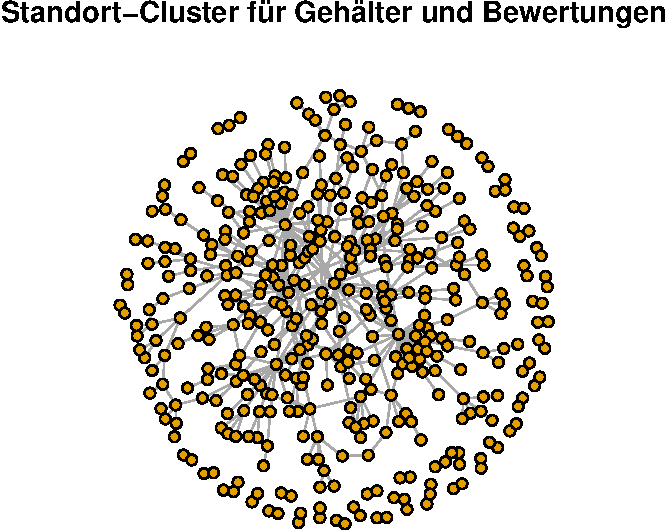
\includegraphics[keepaspectratio]{DataScience_files/figure-latex/unnamed-chunk-20-1.pdf}}

\subsubsection{Degree-Zentralität}\label{degree-zentralituxe4t}

Hier wird die Anzahl der Kanten gezählt, die an jedem Knoten hängen.
Hohe Werte können auf starke Verbindungen zu anderen Unternehmen
hinweisen.

Ein Unternehmen mit einer hohen Degree-Zentralität ist in der Regel gut
vernetzt und könnte in der Lage sein, bessere Gehälter zu zahlen, um
Talente anzuziehen.

\begin{Shaded}
\begin{Highlighting}[]
\CommentTok{\# Berechne die Degree{-}Centrality und sortiere sie absteigend}
\NormalTok{top\_degree }\OtherTok{\textless{}{-}} \FunctionTok{head}\NormalTok{(}\FunctionTok{sort}\NormalTok{(degree\_centrality, }\AttributeTok{decreasing =} \ConstantTok{TRUE}\NormalTok{), }\DecValTok{5}\NormalTok{)}

\CommentTok{\# Erstelle ein DataFrame mit den Namen der Unternehmen und ihrer Degree{-}Centrality}
\NormalTok{top\_degree\_df }\OtherTok{\textless{}{-}} \FunctionTok{data.frame}\NormalTok{(}
  \AttributeTok{Company =} \FunctionTok{names}\NormalTok{(top\_degree),}
  \AttributeTok{Degree =} \FunctionTok{as.numeric}\NormalTok{(top\_degree),}
  \AttributeTok{stringsAsFactors =} \ConstantTok{FALSE}
\NormalTok{)}

\CommentTok{\# Erstelle die Tabelle und zentriere sie links}
\FunctionTok{kable}\NormalTok{(top\_degree\_df, }\AttributeTok{format =} \StringTok{"latex"}\NormalTok{, }\AttributeTok{booktabs =} \ConstantTok{TRUE}\NormalTok{, }\AttributeTok{align =} \StringTok{"l"}\NormalTok{) }\SpecialCharTok{\%\textgreater{}\%}
  \FunctionTok{kable\_styling}\NormalTok{(}\AttributeTok{latex\_options =} \FunctionTok{c}\NormalTok{(}\StringTok{"striped"}\NormalTok{, }\StringTok{"hold\_position"}\NormalTok{), }\AttributeTok{position =} \StringTok{"left"}\NormalTok{)}
\end{Highlighting}
\end{Shaded}

\begin{tabular}{ll}
\toprule
Company & Degree\\
\midrule
\cellcolor{gray!10}{Accenture} & \cellcolor{gray!10}{7}\\
AstraZeneca & 5\\
\cellcolor{gray!10}{Infosys} & \cellcolor{gray!10}{5}\\
Booz Allen Hamilton & 5\\
\cellcolor{gray!10}{BioMarin Pharmaceutical} & \cellcolor{gray!10}{4}\\
\bottomrule
\end{tabular}

\subsubsection{Eigenvector-Zentralität}\label{eigenvector-zentralituxe4t}

\begin{Shaded}
\begin{Highlighting}[]
\CommentTok{\# Berechne die Eigenvector{-}Centrality und sortiere sie absteigend}
\NormalTok{top\_eigenvector }\OtherTok{\textless{}{-}} \FunctionTok{head}\NormalTok{(}\FunctionTok{sort}\NormalTok{(eigenvector\_centrality, }\AttributeTok{decreasing =} \ConstantTok{TRUE}\NormalTok{), }\DecValTok{5}\NormalTok{)}

\CommentTok{\# Erstelle ein DataFrame mit den Namen der Unternehmen und ihrer Eigenvector{-}Centrality}
\NormalTok{top\_eigenvector\_df }\OtherTok{\textless{}{-}} \FunctionTok{data.frame}\NormalTok{(}
  \AttributeTok{Company =} \FunctionTok{names}\NormalTok{(top\_eigenvector),}
  \AttributeTok{Eigenvector =} \FunctionTok{as.numeric}\NormalTok{(top\_eigenvector),}
  \AttributeTok{stringsAsFactors =} \ConstantTok{FALSE}
\NormalTok{)}

\CommentTok{\# Erstelle die Tabelle und zentriere sie links}
\FunctionTok{kable}\NormalTok{(top\_eigenvector\_df, }\AttributeTok{format =} \StringTok{"latex"}\NormalTok{, }\AttributeTok{booktabs =} \ConstantTok{TRUE}\NormalTok{, }\AttributeTok{align =} \StringTok{"l"}\NormalTok{) }\SpecialCharTok{\%\textgreater{}\%}
  \FunctionTok{kable\_styling}\NormalTok{(}\AttributeTok{latex\_options =} \FunctionTok{c}\NormalTok{(}\StringTok{"striped"}\NormalTok{, }\StringTok{"hold\_position"}\NormalTok{), }\AttributeTok{position =} \StringTok{"left"}\NormalTok{)}
\end{Highlighting}
\end{Shaded}

\begin{tabular}{ll}
\toprule
Company & Eigenvector\\
\midrule
\cellcolor{gray!10}{Takeda Pharmaceuticals} & \cellcolor{gray!10}{1.0000000}\\
Novartis & 0.6885416\\
\cellcolor{gray!10}{Pfizer} & \cellcolor{gray!10}{0.5750772}\\
Baxter & 0.5510613\\
\cellcolor{gray!10}{AstraZeneca} & \cellcolor{gray!10}{0.3694600}\\
\bottomrule
\end{tabular}

\subsection{Cluster-Analyse}\label{cluster-analyse}

Klassifizierung der Unternehmen: Unternehmen werden basierend auf ihrer
Netzwerkposition in zentrale (innerhalb von Netzwerken) und periphere
(am Rand der Netzwerke) Gruppen klassifiziert. Gehaltsvergleich:
Verwende Boxplots oder Histogramme, um die Gehaltsverteilung in beiden
Gruppen zu vergleichen. Beispiel: „Die Boxplots zeigen, dass die
medianen Gehälter in zentralen Positionen signifikant höher sind als in
peripheren Positionen.``

Abschließend soll noch eine Clusteranalyse durchgeführt werden, die die
Gehalt in Bezug auf Standort und Wettbewerb kombiniert betrachtet.
\#\#\# Cluster-Analyse Clusteranalyse innerhalb des geografischen und
Wettbewerbsnetzwerks. Cluster von Unternehmen nach Gehalt und Standort
innerhalb des Wettbewerbsnetzwerks: Korrelation zwischen Gehältern und
der Stärke von Wettbewerb und regionaler Vernetzung. Regionale
Gehaltsklassen: Visualisierung der regionalen Gehaltsspreizung in Bezug
auf Netzwerkcluster, z.B. ob Cluster in wirtschaftsstarken Regionen
höhere Durchschnittsgehälter bieten.

\begin{Shaded}
\begin{Highlighting}[]
\CommentTok{\# Detect communities}
\NormalTok{communities }\OtherTok{\textless{}{-}} \FunctionTok{cluster\_louvain}\NormalTok{(g\_direct\_competitors)}
\end{Highlighting}
\end{Shaded}

Vllt: bevor wir mit den Clustern loslegen TODO ``Arc Diagramm'' zu den
regionalen Clustern von der geografischen Netzwerkanalyse

\subsection{Ergänzung zu den
Zentralitätsanalysen}\label{erguxe4nzung-zu-den-zentralituxe4tsanalysen}

\begin{Shaded}
\begin{Highlighting}[]
\CommentTok{\# Prepare data for visNetwork}
\NormalTok{nodes }\OtherTok{\textless{}{-}} \FunctionTok{data.frame}\NormalTok{(}\AttributeTok{id =} \FunctionTok{V}\NormalTok{(g\_direct\_competitors)}\SpecialCharTok{$}\NormalTok{name,}
                    \AttributeTok{label =} \FunctionTok{V}\NormalTok{(g\_direct\_competitors)}\SpecialCharTok{$}\NormalTok{name,}
                    \AttributeTok{group =} \FunctionTok{membership}\NormalTok{(communities),}
                    \AttributeTok{value =}\NormalTok{ degree\_centrality,}
                    \AttributeTok{title =} \FunctionTok{paste}\NormalTok{(}\StringTok{"Degree:"}\NormalTok{, degree\_centrality, }
                                  \StringTok{"\textless{}br\textgreater{}Betweenness:"}\NormalTok{, betweenness\_centrality, }
                                  \StringTok{"\textless{}br\textgreater{}Closeness:"}\NormalTok{, closeness\_centrality, }
                                  \StringTok{"\textless{}br\textgreater{}Eigenvector:"}\NormalTok{, eigenvector\_centrality))}

\NormalTok{edges }\OtherTok{\textless{}{-}} \FunctionTok{data.frame}\NormalTok{(}\AttributeTok{from =} \FunctionTok{as.character}\NormalTok{(edges}\SpecialCharTok{$}\NormalTok{from), }\AttributeTok{to =} \FunctionTok{as.character}\NormalTok{(edges}\SpecialCharTok{$}\NormalTok{to))}

\CommentTok{\# Create interactive network visualization}
\FunctionTok{visNetwork}\NormalTok{(nodes, edges) }\SpecialCharTok{\%\textgreater{}\%}
  \FunctionTok{visOptions}\NormalTok{(}\AttributeTok{highlightNearest =} \ConstantTok{TRUE}\NormalTok{, }\AttributeTok{nodesIdSelection =} \ConstantTok{TRUE}\NormalTok{) }\SpecialCharTok{\%\textgreater{}\%}
  \FunctionTok{visGroups}\NormalTok{(}\AttributeTok{groupname =} \StringTok{"1"}\NormalTok{, }\AttributeTok{color =} \StringTok{"red"}\NormalTok{) }\SpecialCharTok{\%\textgreater{}\%}
  \FunctionTok{visGroups}\NormalTok{(}\AttributeTok{groupname =} \StringTok{"2"}\NormalTok{, }\AttributeTok{color =} \StringTok{"blue"}\NormalTok{) }\SpecialCharTok{\%\textgreater{}\%}
  \FunctionTok{visGroups}\NormalTok{(}\AttributeTok{groupname =} \StringTok{"3"}\NormalTok{, }\AttributeTok{color =} \StringTok{"green"}\NormalTok{) }\SpecialCharTok{\%\textgreater{}\%}
  \FunctionTok{visGroups}\NormalTok{(}\AttributeTok{groupname =} \StringTok{"4"}\NormalTok{, }\AttributeTok{color =} \StringTok{"yellow"}\NormalTok{) }\SpecialCharTok{\%\textgreater{}\%}
  \FunctionTok{visGroups}\NormalTok{(}\AttributeTok{groupname =} \StringTok{"5"}\NormalTok{, }\AttributeTok{color =} \StringTok{"purple"}\NormalTok{) }\SpecialCharTok{\%\textgreater{}\%}
  \FunctionTok{visGroups}\NormalTok{(}\AttributeTok{groupname =} \StringTok{"6"}\NormalTok{, }\AttributeTok{color =} \StringTok{"orange"}\NormalTok{) }\SpecialCharTok{\%\textgreater{}\%}
  \FunctionTok{visGroups}\NormalTok{(}\AttributeTok{groupname =} \StringTok{"7"}\NormalTok{, }\AttributeTok{color =} \StringTok{"pink"}\NormalTok{) }\SpecialCharTok{\%\textgreater{}\%}
  \FunctionTok{visLayout}\NormalTok{(}\AttributeTok{randomSeed =} \DecValTok{123}\NormalTok{) }\SpecialCharTok{\%\textgreater{}\%}
  \FunctionTok{visLegend}\NormalTok{()}
\end{Highlighting}
\end{Shaded}

\pandocbounded{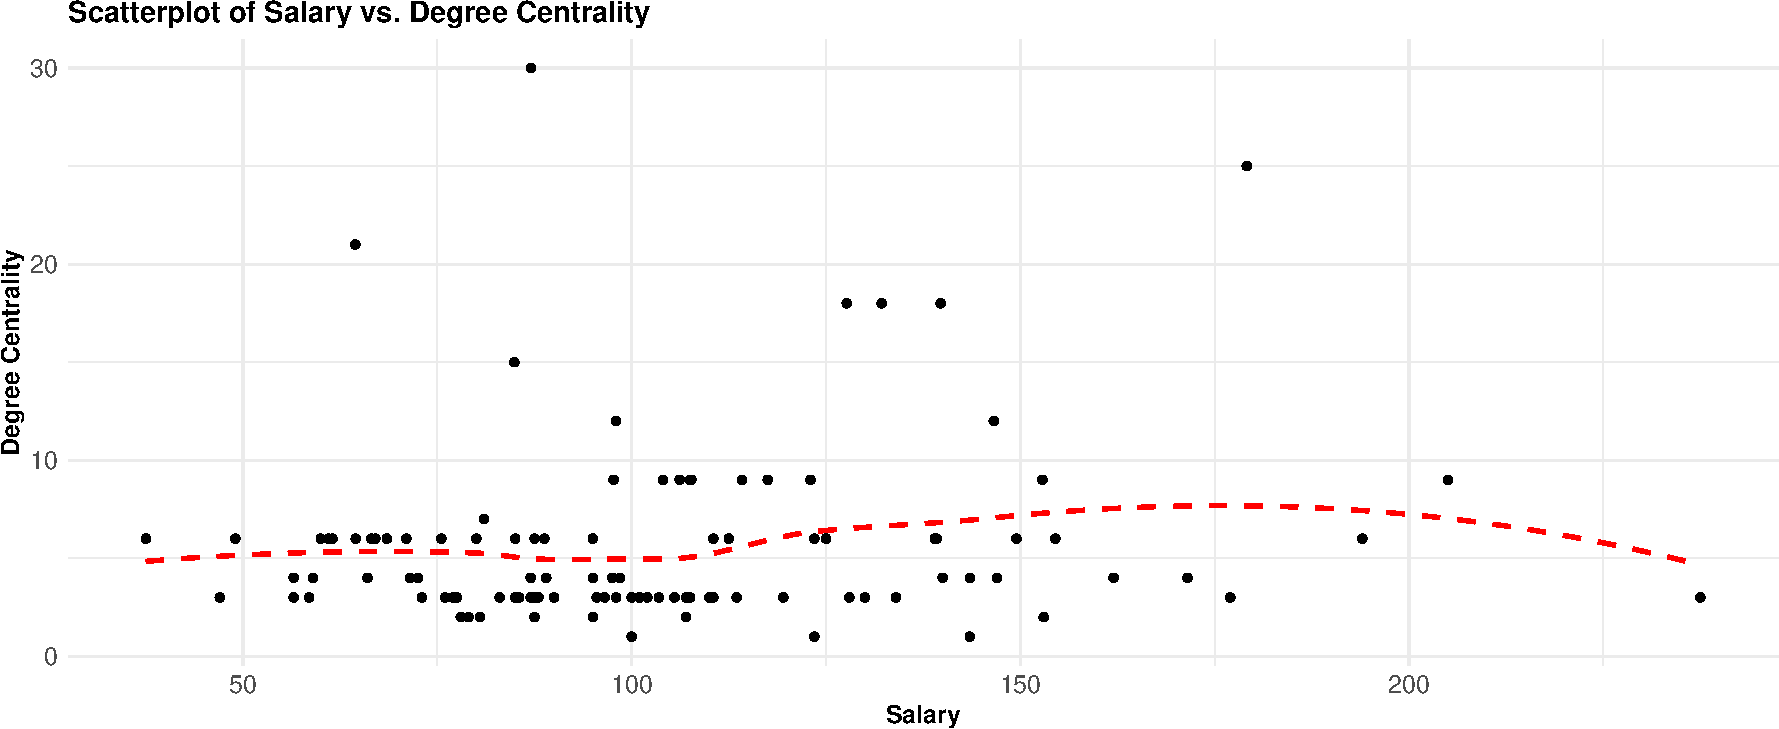
\includegraphics[keepaspectratio]{DataScience_files/figure-latex/unnamed-chunk-24-1.pdf}}

\begin{Shaded}
\begin{Highlighting}[]
\CommentTok{\# Fügt ein Bild der interaktiven Netzwerkvisualisierung hinzu}
\NormalTok{knitr}\SpecialCharTok{::}\FunctionTok{include\_graphics}\NormalTok{(}\StringTok{"interaktive\_Netzwerke\_Bilder/Übersicht.png"}\NormalTok{)}
\end{Highlighting}
\end{Shaded}

\pandocbounded{\includegraphics[keepaspectratio]{interaktive_Netzwerke_Bilder/Übersicht.png}}

\begin{Shaded}
\begin{Highlighting}[]
\NormalTok{knitr}\SpecialCharTok{::}\FunctionTok{include\_graphics}\NormalTok{(}\StringTok{"interaktive\_Netzwerke\_Bilder/NVDIA.png"}\NormalTok{)}
\end{Highlighting}
\end{Shaded}

\pandocbounded{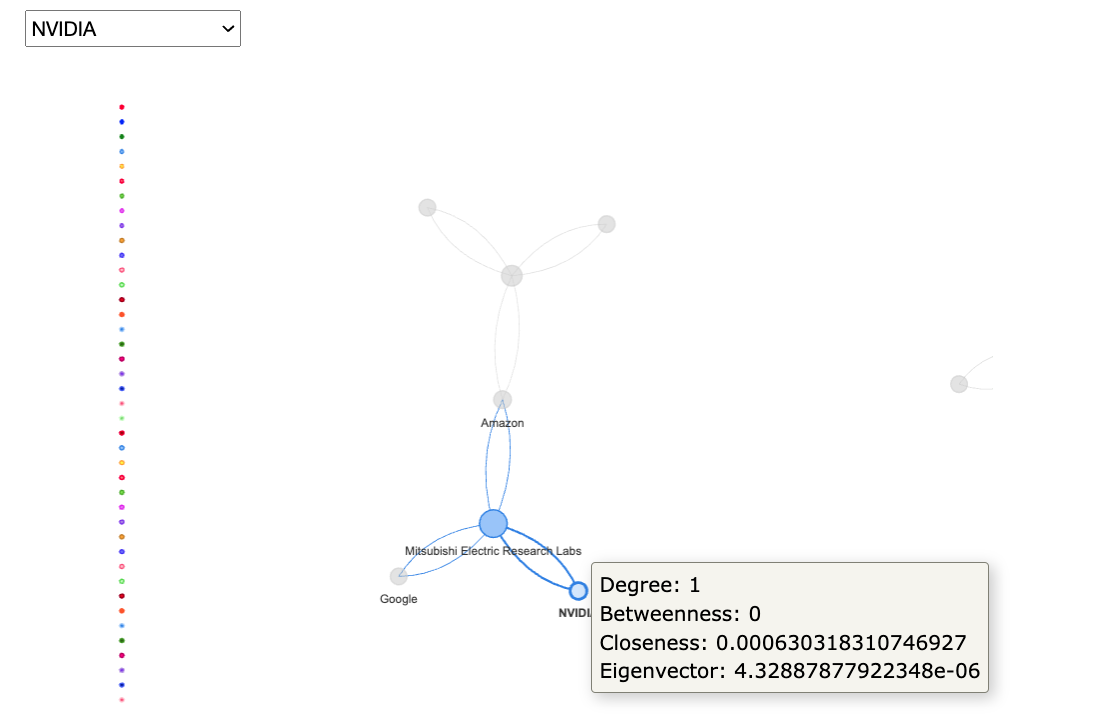
\includegraphics[keepaspectratio]{interaktive_Netzwerke_Bilder/NVDIA.png}}
Zugriff auf die interaktive Visualisierung über das Repository
(Dateiname: network.html): \url{https://github.com/Mzaex7/SNA}

\newpage

\section{Conclusion}\label{conclusion}

Zusammenfassung der zentralen Ergebnisse:

Bedeutung: Diskutiere, wie wichtig geografische Nähe und
Wettbewerbsumfeld für die Karriereentwicklung von Data Scientists sind.

Praktische Implikationen: Gib Empfehlungen für Jobuchende, wie sie
Standorte und Unternehmen auswählen sollten, um die besten
Gehaltsaussichten zu haben. Dies könnte auch für Unternehmen von
Interesse sein, um zu verstehen, wie sie ihre Position im Markt
verbessern können.

\newpage

\section{Literaturverzeichnis}\label{literaturverzeichnis}

Davenport, Thomas H.; Patil, D. J. 2012. »Data Scientist: The Sexiest
Job of the 21st Century«, in Harvard Business Review vom 1. Oktober
2012.
\url{https://hbr.org/2012/10/data-scientist-the-sexiest-job-of-the-21st-century}
(Zugriff vom 30.10.2024).

Google Trends,
\url{https://trends.google.com/trends/explore?date=all&q=\%22data\%20science\%22,\%22data\%20scientist\%22}
(Zugriff vom 30.10.2024).

\end{document}
